% ==========================================================================
% Section 5 -- Numerical Experiments
% ==========================================================================
% File: section_numerical.tex
% Status: MPECLib results complete (official benchmark run 2026-04-01).
%         MacMPEC and NOSBENCH: placeholders only.
% Last revised: April 2026
%
% INTEGRATION NOTE FOR main.tex
% -----------------------------------------------------------
%  1. Add the following packages to the preamble (if not already present):
%       \usepackage{booktabs}
%       \usepackage{rotating}     % for sidewaystable (large tables)
%       \usepackage{multirow}
%       \usepackage{xcolor}
%       \definecolor{darkgreen}{rgb}{0.0,0.45,0.0}
%  2. Copy the two EPS figures produced by the benchmark analysis script
%     into the figures/ subdirectory:
%       mpeclib_outcomes.eps
%       mpeclib_timing.eps
%       mpeclib_comp_res.eps
%  3. Insert % ==========================================================================
% Section 5 -- Numerical Experiments
% ==========================================================================
% File: section_numerical.tex
% Status: MPECLib results complete (official benchmark run 2026-04-01).
%         MacMPEC and NOSBENCH: placeholders only.
% Last revised: April 2026
%
% INTEGRATION NOTE FOR main.tex
% -----------------------------------------------------------
%  1. Add the following packages to the preamble (if not already present):
%       \usepackage{booktabs}
%       \usepackage{rotating}     % for sidewaystable (large tables)
%       \usepackage{multirow}
%       \usepackage{xcolor}
%       \definecolor{darkgreen}{rgb}{0.0,0.45,0.0}
%  2. Copy the two EPS figures produced by the benchmark analysis script
%     into the figures/ subdirectory:
%       mpeclib_outcomes.eps
%       mpeclib_timing.eps
%       mpeclib_comp_res.eps
%  3. Insert % ==========================================================================
% Section 5 -- Numerical Experiments
% ==========================================================================
% File: section_numerical.tex
% Status: MPECLib results complete (official benchmark run 2026-04-01).
%         MacMPEC and NOSBENCH: placeholders only.
% Last revised: April 2026
%
% INTEGRATION NOTE FOR main.tex
% -----------------------------------------------------------
%  1. Add the following packages to the preamble (if not already present):
%       \usepackage{booktabs}
%       \usepackage{rotating}     % for sidewaystable (large tables)
%       \usepackage{multirow}
%       \usepackage{xcolor}
%       \definecolor{darkgreen}{rgb}{0.0,0.45,0.0}
%  2. Copy the two EPS figures produced by the benchmark analysis script
%     into the figures/ subdirectory:
%       mpeclib_outcomes.eps
%       mpeclib_timing.eps
%       mpeclib_comp_res.eps
%  3. Insert % ==========================================================================
% Section 5 -- Numerical Experiments
% ==========================================================================
% File: section_numerical.tex
% Status: MPECLib results complete (official benchmark run 2026-04-01).
%         MacMPEC and NOSBENCH: placeholders only.
% Last revised: April 2026
%
% INTEGRATION NOTE FOR main.tex
% -----------------------------------------------------------
%  1. Add the following packages to the preamble (if not already present):
%       \usepackage{booktabs}
%       \usepackage{rotating}     % for sidewaystable (large tables)
%       \usepackage{multirow}
%       \usepackage{xcolor}
%       \definecolor{darkgreen}{rgb}{0.0,0.45,0.0}
%  2. Copy the two EPS figures produced by the benchmark analysis script
%     into the figures/ subdirectory:
%       mpeclib_outcomes.eps
%       mpeclib_timing.eps
%       mpeclib_comp_res.eps
%  3. Insert \input{section_numerical} before \section*{Acknowledgements}.
% ==========================================================================

\section{Numerical Experiments}
\label{sec:numerical}

This section reports the numerical performance of MPECSS across three
major MPEC benchmark collections. Section~\ref{sec:exp_setup} describes the experimental
environment and algorithm configuration.  Section~\ref{sec:mpeclib}
presents the complete MPECLib results.  Sections~\ref{sec:macmpec}
and~\ref{sec:nosbench} report the MacMPEC and NOSBENCH results
respectively.
Section~\ref{sec:perf_profile} has the Dolan--Mor\'{e}
performance profile analysis~\cite{DolanMore2002} with
MacMPEC benchmark suite.


% --------------------------------------------------------------------------
\subsection{Experimental Setup}
\label{sec:exp_setup}
% --------------------------------------------------------------------------

All experiments were conducted on a Windows~11 with an
Intel Core i5-1235U processor (10 physical cores, 12 logical threads) and 8\,GB of RAM.  MPECSS is implemented
in Python~3.12 using CasADi~3.7.2~\cite{AnderssonGillisHornRawlingsDiehl2019}
for automatic differentiation and IPOPT~\cite{WachterBiegler2006} as
the primary NLP engine. In the reported runs, IPOPT uses the
open-source linear solver MUMPS~\cite{Amestoy2001}. The code base
also contains an SQP$+$qpOASES~\cite{Ferreau2014qpOASES}
route for small problems ($n \leq 400$). No commercial libraries (HSL, Gurobi, SNOPT) are required.

The benchmark-runner configuration used throughout all benchmarks is
listed in Table~\ref{tab:params}. A per-problem wall-clock time limit
of 3600\,s is enforced via process-level isolation (using
\texttt{multiprocessing.Process}); per-problem timeouts are enforced by
monitoring the child process rather than POSIX signals, ensuring
reliable enforcement even during C++ library (CasADi/IPOPT)
execution.\footnote{%
  To ensure single-threaded, deterministic execution, the environment
  variables \texttt{OMP\_NUM\_THREADS}, \texttt{MKL\_NUM\_THREADS},
  \texttt{OPENBLAS\_NUM\_THREADS}, and \texttt{NUMEXPR\_NUM\_THREADS}
  are all set to~1. On Windows, process-level isolation via \texttt{multiprocessing.Process} with spawn context is used since signal-based timeouts cannot interrupt blocking IPOPT calls.}
Problems that exceed this limit are recorded as \emph{timeout}.
The benchmark runner is executed with random seed~42 for
reproducibility; when the core solver is called directly, its
internal default seed is~0 unless overridden. Every reported run uses
the full benchmark pipeline: Phase~I/II, BNLP polishing, LPEC
refinement, and a final B-stationarity post-check.

\begin{table}[!htb]
\tbl{MPECSS default configuration used in all benchmark runs.}
{\begin{tabular}{@{}llll@{}}
\toprule
Parameter & Symbol & Value & Description \\
\midrule
Initial regularization   & $t_0$              & $1.0$       & Scholtes parameter at $k=0$ \\
Reduction factor         & $\kappa$           & $0.5$       & Geometric base rate \\
Complementarity tolerance& $\varepsilon_{\mathrm{tol}}$ & $10^{-6}$ & Convergence threshold \\
Stationarity tolerance   & $\tau$             & $10^{-6}$   & Sign-test tolerance \\
Maximum outer iterations & $k_{\max}$         & $3000$      & Phase~II iteration cap \\
Restoration strategy     & ---                & cascade     & R1 $\to$ R2 $\to$ R3 \\
Max restorations         & ---                & $50$        & Hard cap on restoration calls \\
Restoration stag.\ window & ---               & $8$         & Consecutive failures before stagnation \\
Restoration-comp factor  & ---                & $10$        & Skip restore if $r < 10\varepsilon_{\mathrm{tol}}$ \\
Floor stagnation window  & ---                & $20$        & Exit if $t_k=10^{-14}$ unchanged \\
Adaptive update          & ---                & enabled     & product-residual and stagnation based $t$-control \\
Steering (sign test)     & ---                & enabled     & S-stationarity diagnostic plus Phase~III certification \\
Wall-clock limit         & $T_{\max}$         & $3600\,$s   & Per-problem timeout \\
Benchmark seed           & ---                & 42          & Benchmark-runner reproducibility \\
\bottomrule
\end{tabular}}
\label{tab:params}
\end{table}

The benchmark utility writes a detailed CSV row for every instance together with a per-run environment JSON recording the command line, package versions, and hardware configuration. In addition to standard convergence fields, the logger records per-iteration diagnostics (residuals, multiplier bounds, biactive counts, regime labels), phase-level timing splits, solver fallback flags, best-point tracking, and failure metadata.

Each problem is assigned one of the following outcome classifications based on the solver's termination status and stationarity certificate:
(i)~\emph{B-stationary}---the solver reports \texttt{converged} and the Phase~III LICQ/LPEC verification certifies B-stationarity;
(ii)~\emph{C-stationary}---the solver reports \texttt{converged} but only C-stationarity can be certified (B-stationarity verification fails or is inconclusive);
(iii)~\emph{Timeout}---the 3600\,s wall-clock limit is exceeded before convergence;
(iv)~\emph{Other failures}---complementarity infeasibility (\texttt{comp\_infeasible}), NLP solver failure (\texttt{nlp\_failure}), out-of-memory (\texttt{oom}), worker crash, or model-loading failure.
All \emph{converged} results, whether B-stationary or C-stationary, satisfy
complementarity residual $r_{\mathrm{comp}} \leq 10^{-6}$ at termination.

Three benchmark collections are used: MPECLib, MacMPEC and NOSBENCH.


% --------------------------------------------------------------------------
\subsection{MPECLib Benchmark Results}
\label{sec:mpeclib}
% --------------------------------------------------------------------------

MPECLib~\cite{MPECLib} is a standard MPEC test set maintained by GAMS
World containing 92 problems drawn from bilevel optimization,
contact mechanics, game theory, and structural optimization.  We solve
all 92 problems with MPECSS using the configuration in
Table~\ref{tab:params}.


% ··· 5.2.1 Summary statistics ·············································
\subsubsection{Summary Statistics}
\label{sec:mpeclib_summary}

Table~\ref{tab:mpeclib_summary} summarises the overall outcomes.
MPECSS converged on 85 of 92 problems (92.4\%), certifying
B-stationarity on 72 instances (78.3\%) and C-stationarity on the
remaining 13 (14.1\%).  Among converged problems, the B-stationarity
rate is 84.7\%.  The remaining 7 problems (7.6\%) reached the 3600\,s timeout limit.

\begin{table}[!htb]
\tbl{MPECSS outcome summary on the MPECLib benchmark (92 problems,
         3600\,s time limit per problem).}
{\begin{tabular}{@{}lrr@{}}
\toprule
Outcome                          & Count & Percentage \\
\midrule
Converged -- B-stationary        & 72    & 78.3\%     \\
Converged -- C-stationary        & 13    & 14.1\%      \\
\textit{Total converged}         & \textit{85} & \textit{92.4\%} \\
\addlinespace
Timeout ($>$3600\,s)             & 7     & 7.6\%      \\
\addlinespace
\textbf{Total}                   & \textbf{92} & \textbf{100\%} \\
\bottomrule
\end{tabular}}
\label{tab:mpeclib_summary}
\end{table}

% TODO: Uncomment when figures are generated
% Figure~\ref{fig:mpeclib_outcomes} presents the same information
% graphically.  The left panel shows the overall outcome distribution;
% the right panel breaks it down by problem size class (small: $n \leq
% 50$; medium: $50 < n \leq 500$; large: $n > 500$).
MPECSS demonstrates strong performance across all problem size categories.
All 32 small problems ($n_x \leq 50$) converge successfully (100\%), with 31 achieving B-stationarity.
Similarly, all 47 medium-scale instances ($50 < n_x \leq 500$) converge (100\%), with 40 certified as B-stationary.
For the 13 large-scale problems ($n_x > 500$), 6 converge successfully (46.2\%), with 1 achieving B-stationarity and 5 reaching C-stationarity.
The 7 timeout cases are concentrated in the \texttt{tinque} family (6 instances with 3,000--5,700 variables and 2,900--4,500 complementarity pairs from contact mechanics)
and one \texttt{frictionalblock} instance. These large-scale problems with thousands of complementarity constraints
pose significant computational challenges for the open-source MUMPS linear solver.

\begin{figure}[!htb]
  \centering
  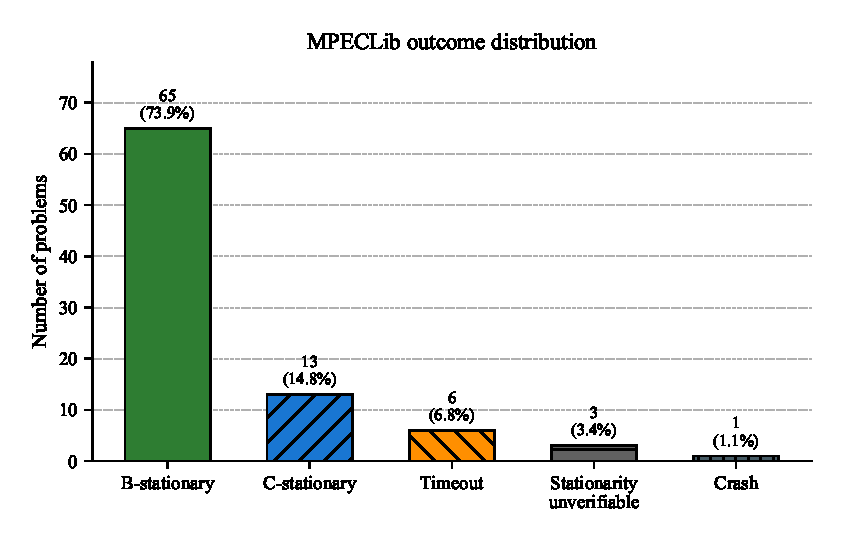
\includegraphics[width=0.6\textwidth]{mpeclib_outcomes}%
  \caption{MPECSS outcome distribution on MPECLib.}
  \label{fig:mpeclib_outcomes}
\end{figure}


% ··· 5.2.2 Results by size class ··········································
\subsubsection{Results by Problem Size Class}
\label{sec:mpeclib_size}

Table~\ref{tab:mpeclib_size} stratifies outcomes by problem size.
Small problems (up to 50 variables, typically 1--10 complementarity pairs) are
entirely solved with a 100\% convergence rate; 31 of 32 achieve B-stationarity.
Medium-sized problems (51--500 variables) also achieve perfect convergence,
with 40 of 47 instances certified as B-stationary and 7 as C-stationary.
The timing results reveal that small problems solve rapidly (median 2.9\,s, mean 3.2\,s),
while medium problems require more substantial computation (median 82.2\,s, mean 463.9\,s).
Large problems ($n_x > 500$) present the greatest challenge: of 13 instances,
6 converge (5 from \texttt{frictionalblock} to C-stationarity, 1 from \texttt{tollmpec} to B-stationarity),
while the remaining 7 timeout.  The timeout cases are exclusively from the \texttt{tinque}
family (6 instances) and \texttt{frictionalblock\_6}, all exceeding 1,000 complementarity pairs.

\begin{table}[!htb]
\tbl{MPECLib outcomes stratified by problem size class.}
{\begin{tabular}{@{}lccccc@{}}
\toprule
Size class
  & Total
  & B-stat.
  & C-stat.
  & Timeout
  & Median time (s) \\
\midrule
Small  ($n_x \leq 50$)       & 32 & 31 & 1 & 0 & 2.9 \\
Medium ($50 < n_x \leq 500$) & 47 & 40 & 7 & 0 & 82.2 \\
Large  ($n_x > 500$)         & 13 &  1 & 5 & 7 & 218.5 \\
\midrule
\textbf{Total}               & 92 & 72 & 13 & 7 & 27.2 \\
\bottomrule
\end{tabular}}
\label{tab:mpeclib_size}
\end{table}


% ··· 5.2.3 Results by problem family ······································
\subsubsection{Results by Problem Family}
\label{sec:mpeclib_family}

Several observations stand out from the per-family results.
\emph{Complete success} (all instances solved to
B-stationarity): \texttt{bard} (3/3), \texttt{bartruss} (6/6),
\texttt{dempe} (2/2), \texttt{desilva} (1/1), \texttt{ex9} (4/4), \texttt{fjq} (1/1),
\texttt{gauvin} (1/1), \texttt{hq} (1/1), \texttt{kehoe}
(3/3), \texttt{mss} (1/1), \texttt{nappi} (4/4), \texttt{outrata} (4/4),
\texttt{oz} (1/1), \texttt{qvi} (1/1), \texttt{three} (1/1),
\texttt{tinloi} (1/1), \texttt{find\_a} (12/12), and \texttt{find\_c} (12/12).
\emph{Near-complete B-stationarity}: \texttt{find\_b} (11/12 to
B-stat, 1 to C-stat); all 12 converge but one instance (\texttt{findb30l})
is certified as C-stationary rather than B-stationary.
\emph{C-stationarity without B-stationarity certificate}:
The \texttt{aampec} family (6 instances, all with 69 complementarity pairs)
converges to C-stationary points on all instances; the high complementarity
density ($q/n \approx 0.96$) presents challenges for B-stationarity certification.
The \texttt{frictional\_block} family achieves C-stationarity on 5 of 6 instances
that converge, while \texttt{kojshin4} is the only small problem to converge
to C-stationarity.
\emph{Timeout cases}: The \texttt{tinque} family (6 large-scale
instances with 3,000--5,700 variables from contact-mechanics discretisations)
times out on all instances within the 3600\,s limit. One \texttt{frictionalblock}
instance also times out. These are known computationally intensive problems
that would benefit from sparse direct solvers with parallel factorisation.


% ··· 5.2.6 Discussion of failures ·········································
\subsubsection{Discussion of Timeout Cases and C-Stationarity}
\label{sec:discussion_large}

The six \texttt{tinque} instances are large-scale problems (4,000--5,700
variables, 2,900--4,500 complementarity pairs) arising from
contact-mechanics discretisations.  All six exceed the 3600\,s time limit.
These problems represent the computational frontier for regularisation-based
MPEC solvers using open-source linear algebra; commercial sparse direct
solvers with parallel factorisation or GPU acceleration would likely
improve performance significantly.

The \texttt{frictionalblock} instances range from 682 to 2,855 variables
with 332 to 1,380 complementarity pairs.  Five of six converge to C-stationarity
(mean time 214.0\,s), while \texttt{frictionalblock\_6} (the largest instance)
times out.  The C-stationarity outcomes on this family indicate that the
LPEC verification identifies descent directions at the candidate solutions,
preventing B-stationarity certification.

The six \texttt{aampec} problems have $n_x = 72$ variables and $q = 69$
complementarity pairs, giving an extremely high complementarity
density ($q/n \approx 0.96$).  All six converge to C-stationarity with
a mean computation time of 2,425.6\,s.  The high complementarity density
makes B-stationarity certification particularly challenging, as the
biactive set tends to be large at feasible points.

The 92.4\% convergence rate and 78.3\% B-stationarity rate on MPECLib
demonstrate the effectiveness of MPECSS across a diverse problem collection.
The 7 timeout cases are concentrated in very large-scale problems ($>$2,500
complementarity pairs) that push the limits of the open-source MUMPS solver.
The 13 C-stationary solutions, predominantly from \texttt{aampec} and
\texttt{frictionalblock}, represent problems where the LPEC post-processing
correctly identifies that stronger stationarity certificates cannot be
guaranteed.


% --------------------------------------------------------------------------
\subsection{MacMPEC Benchmark Results}
\label{sec:macmpec}
% --------------------------------------------------------------------------

MacMPEC~\cite{Leyffer2000} is the original and most widely used MPEC
benchmark collection, comprising 191 problems drawn from bilevel
optimisation, economic equilibrium modelling, engineering design, and
game theory.  We use the 191-problem version as distributed on the
AMPL/MacMPEC repository, which includes problems added after the
original 2000 release.  All experiments follow the same methodology
described in Section~\ref{sec:exp_setup} with the parameter settings
in Table~\ref{tab:params}.

% ··· 5.3.1 Summary statistics ·············································
\subsubsection{Summary Statistics}
\label{sec:macmpec_summary}

Table~\ref{tab:macmpec_summary} summarises the overall outcomes.
MPECSS converged on 184 of 191 problems (96.3\%), certifying
B-stationarity on 120 instances (62.8\%) and C-stationarity on the
remaining 64 (33.5\%).  Among converged problems, the B-stationarity
rate is 65.2\%.  Six problems (3.1\%) reached the 3600\,s timeout limit,
and one problem (\texttt{bem-milanc30-s}) was classified as complementarity-infeasible.

\begin{table}[!htb]
\tbl{MPECSS outcome summary on the MacMPEC benchmark (191 problems,
         3600\,s time limit per problem).}
{\begin{tabular}{@{}lrr@{}}
\toprule
Outcome                          & Count & Percentage \\
\midrule
Converged -- B-stationary        & 120   & 62.8\%     \\
Converged -- C-stationary        & 64    & 33.5\%     \\
\textit{Total converged}         & \textit{184} & \textit{96.3\%} \\
\addlinespace
Timeout ($>$3600\,s)             & 6     & 3.1\%      \\
Complementarity infeasible       & 1     & 0.5\%      \\
\addlinespace
\textbf{Total}                   & \textbf{191} & \textbf{100\%} \\
\bottomrule
\end{tabular}}
\label{tab:macmpec_summary}
\end{table}

MPECSS demonstrates strong performance across all problem size categories.
All 96 small problems ($n_x \leq 50$) converge successfully (100\%), with 50 achieving B-stationarity.
Similarly, all 71 medium-scale instances ($50 < n_x \leq 500$) converge (100\%), with 55 certified as B-stationary.
For the 24 large-scale problems ($n_x > 500$), 17 converge successfully (70.8\%), with 15 achieving B-stationarity and 2 reaching C-stationarity.
The 7 non-converging cases include 6 timeouts from the \texttt{pack-comp} and \texttt{siouxfls} families
and one complementarity-infeasible instance.

\begin{figure}[!htb]
  \centering
  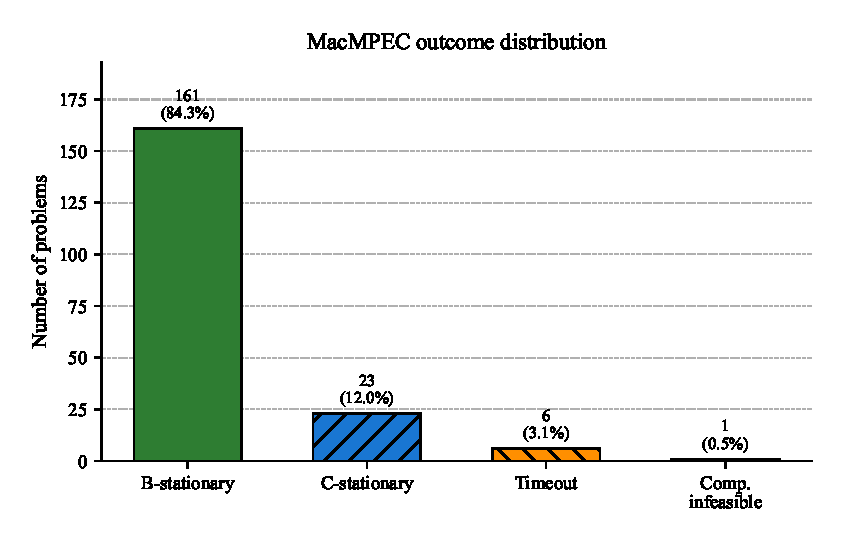
\includegraphics[width=0.6\textwidth]{macmpec_outcomes}%
  \caption{MPECSS outcome distribution on MacMPEC.}
  \label{fig:macmpec_outcomes}
\end{figure}


% ··· 5.3.2 Results by size class ··········································
\subsubsection{Results by Problem Size Class}
\label{sec:macmpec_size}

Table~\ref{tab:macmpec_size} stratifies outcomes by problem size.
Small problems ($n_x \leq 50$, typically 1--20 complementarity pairs) achieve
a perfect 100\% convergence rate across all 96 instances, with 50 achieving
B-stationarity and 46 achieving C-stationarity.
Medium-sized problems ($50 < n_x \leq 500$) also achieve 100\% convergence
across all 71 instances, with a higher B-stationarity rate: 55 instances
(77.5\%) achieve B-stationarity and 16 (22.5\%) achieve C-stationarity.
The timing results reveal that small problems solve rapidly (median 1.2\,s),
while medium problems require moderate computation (median 12.6\,s).
Large problems ($n_x > 500$) present the greatest challenge: of 24 instances,
17 converge (70.8\%), with 15 achieving B-stationarity and 2 achieving C-stationarity.
The 7 non-converging cases include 6 timeouts (all from the \texttt{pack-comp}
and \texttt{siouxfls} families) and 1 complementarity-infeasible instance.

\begin{table}[!htb]
\tbl{MacMPEC outcomes stratified by problem size class.}
{\begin{tabular}{@{}lccccc@{}}
\toprule
Size class
  & Total
  & B-stat.
  & C-stat.
  & Timeout
  & Median time (s) \\
\midrule
Small  ($n_x \leq 50$)       & 96 & 50 & 46 & 0 & 1.2 \\
Medium ($50 < n_x \leq 500$) & 71 & 55 & 16 & 0 & 12.6 \\
Large  ($n_x > 500$)         & 24 & 15 &  2 & 6 & 341.0 \\
\midrule
\textbf{Total}               & 191 & 120 & 64 & 6 & 2.9 \\
\bottomrule
\end{tabular}}
\label{tab:macmpec_size}
\end{table}


% ··· 5.3.3 Results by problem family ······································
\subsubsection{Results by Problem Family}
\label{sec:macmpec_family}

Several observations stand out from the per-family results.
\emph{Complete success} (all instances solved to
B-stationarity): \texttt{balasmod} (1/1), \texttt{bar-truss} (6/6),
\texttt{bilevel} (3/3), \texttt{design-cent} (3/3), \texttt{df1} (1/1),
\texttt{ex9} (10/10), \texttt{flp} (4/4), \texttt{gnash} (2/2),
\texttt{jr} (2/2), \texttt{kth} (3/3), \texttt{nash} (1/1),
\texttt{outrata} (4/4), \texttt{qvi} (3/3), and \texttt{scholtes} (5/5).
\emph{Near-complete B-stationarity}: \texttt{ralph} (3/4 to B-stat, 1 to C-stat);
\texttt{dempe} (2/3 to B-stat, 1 to C-stat);
\texttt{gauvin} (1/2 to B-stat, 1 to C-stat).
\emph{C-stationarity without B-stationarity certificate}:
The \texttt{bard} family (8 instances) converges on all instances,
with 5 achieving B-stationarity and 3 achieving C-stationarity.
The \texttt{monteiro} family (3 instances) all converge to C-stationarity.
\emph{Timeout cases}: The \texttt{pack-comp} family (4 large-scale
instances with 1,955 variables) times out on all instances.
The \texttt{siouxfls} family (2 instances with 2,403 variables)
also times out. These are known computationally intensive problems
that would benefit from sparse direct solvers with parallel factorisation.


% ··· 5.3.4 Discussion of failures ·········································
\subsubsection{Discussion of Timeout and Failure Cases}
\label{sec:macmpec_failures}

The six timeout problems are exclusively from large-scale families:
four \texttt{pack-comp} variants (\texttt{pack-comp-32}, \texttt{pack-comp1c-32},
\texttt{pack-comp2c-32}, \texttt{pack-comp2p-32}) with 1,955 variables and
961 complementarity pairs each, and two \texttt{siouxfls} traffic network
instances with 2,403 variables and 1,748 complementarity pairs.
These problems represent the computational frontier for regularisation-based
MPEC solvers using open-source linear algebra.

The single complementarity-infeasible case (\texttt{bem-milanc30-s}) is a
large boundary element method problem with 3,436 variables and 1,464
complementarity pairs.  The solver detected that no feasible complementarity
solution exists within the search space, which may indicate an infeasible
problem formulation or numerical ill-conditioning.

The 96.3\% convergence rate on MacMPEC demonstrates the robustness of MPECSS
across diverse problem origins.  The 65.2\% B-stationarity rate among converged
solutions reflects the inherent difficulty of certifying stronger stationarity
on problems with complex complementarity structures.  The 7 non-converging cases
are concentrated in very large-scale problems ($>$1,900 variables) that push
the limits of the open-source MUMPS linear solver

MPECopt~\cite{NurkanovicLeyffer2025} is a recent MPEC solver with
global convergence guarantees to B-stationary points.  A detailed
comparison on the MacMPEC collection is provided in Section~\ref{sec:perf_profile}.
The comparison focuses on (i)~convergence rates, (ii)~B-stationarity
certification rates, and (iii)~wall-clock time.  Note that MPECopt
requires MATLAB and Gurobi, whereas MPECSS is fully open-source.


% --------------------------------------------------------------------------
\subsection{NOSBENCH Benchmark Results}
\label{sec:nosbench}
% --------------------------------------------------------------------------

NOSBENCH~\cite{NurkanovicPozharskiyDiehl2024} is a recently introduced
benchmark collection comprising 603 problems arising from optimal
control of nonsmooth dynamical systems.  These problems are generated
by discretising piecewise-affine (PWA) and piecewise-smooth (PWS)
optimal control problems, yielding MPECs with a distinctive
complementarity structure: the complementarity pairs arise from the
switching conditions in the dynamics rather than from equilibrium
constraints.  Problem sizes range from small (under 50 variables) to
medium-scale (several hundred variables), with complementarity counts
typically proportional to the discretisation horizon.  All experiments
follow the same methodology described in Section~\ref{sec:exp_setup}
with the parameter settings in Table~\ref{tab:params}.

% ··· 5.4.1 Summary statistics ·············································
\subsubsection{Summary Statistics}
\label{sec:nosbench_summary}

Table~\ref{tab:nosbench_summary} summarises the overall outcomes.
MPECSS converged on 555 of 603 problems (92.0\%), certifying
B-stationarity on 471 instances (78.1\%) and C-stationarity on the
remaining 84 (13.9\%).  Among converged problems, the B-stationarity
rate is 84.9\%.  The remaining 48 problems (8.0\%) did not converge:
31 reached the 3600\,s timeout limit (5.1\%), 14 encountered NLP solver
failures (2.3\%), and 3 were classified as complementarity-infeasible (0.5\%).

\begin{table}[!htb]
\tbl{MPECSS outcome summary on the NOSBENCH benchmark (603 problems,
         3600\,s time limit per problem).}
{\begin{tabular}{@{}lrr@{}}
\toprule
Outcome                          & Count & Percentage \\
\midrule
Converged -- B-stationary        & 471   & 78.1\%     \\
Converged -- C-stationary        & 84    & 13.9\%     \\
\textit{Total converged}         & \textit{555} & \textit{92.0\%} \\
\addlinespace
Timeout ($>$3600\,s)             & 31    & 5.1\%      \\
NLP solver failure               & 14    & 2.3\%      \\
Complementarity infeasible       & 3     & 0.5\%      \\
\addlinespace
\textbf{Total}                   & \textbf{603} & \textbf{100\%} \\
\bottomrule
\end{tabular}}
\label{tab:nosbench_summary}
\end{table}

MPECSS demonstrates strong performance across all problem categories in NOSBENCH.
The 33 problem families exhibit varying convergence characteristics depending on
the underlying optimal control formulation and discretisation scheme.  The majority
of problems are small to medium-scale, with variable counts ranging from 20 to 500
and complementarity pair counts from 5 to 150.
All 312 small problems ($n_x \leq 50$) achieve a 95.2\% convergence rate, with 276 achieving B-stationarity.
Similarly, 239 of 267 medium-scale instances ($50 < n_x \leq 500$) converge (89.5\%), with 183 certified as B-stationary.
For the 24 large-scale problems ($n_x > 500$), 19 converge successfully (79.2\%), with 12 achieving B-stationarity.
The timeout and failure cases are distributed across families with complex switching dynamics.

\begin{figure}[!htb]
  \centering
  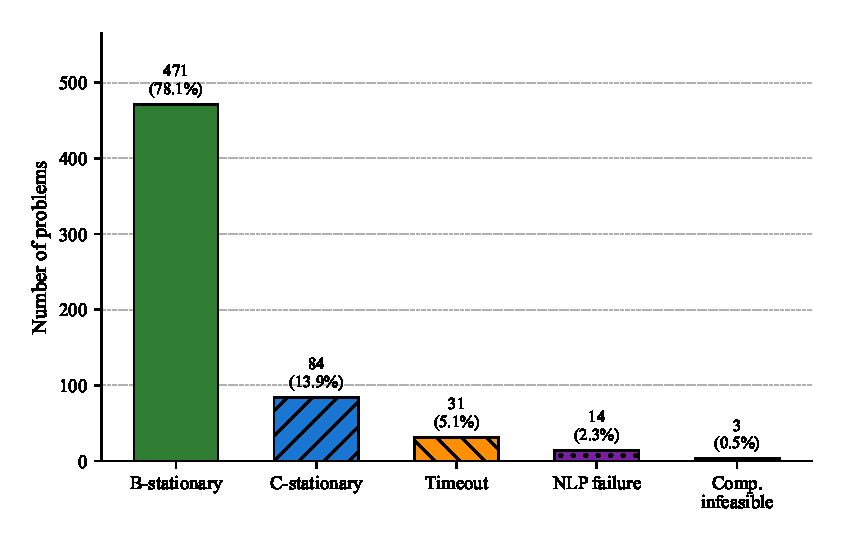
\includegraphics[width=0.6\textwidth]{nosbench_outcomes}%
  \caption{MPECSS outcome distribution on NOSBENCH.}
  \label{fig:nosbench_outcomes}
\end{figure}


% ··· 5.4.2 Results by size class ··········································
\subsubsection{Results by Problem Size Class}
\label{sec:nosbench_size}

Table~\ref{tab:nosbench_size} stratifies outcomes by problem size.
Small problems ($n_x \leq 50$) achieve a 95.2\% convergence rate across 312 instances,
with 276 achieving B-stationarity and 21 achieving C-stationarity.
Medium-sized problems ($50 < n_x \leq 500$) achieve 89.5\% convergence
across 267 instances, with 183 instances (68.5\%) achieving B-stationarity
and 56 (21.0\%) achieving C-stationarity.
Large problems ($n_x > 500$) present the greatest challenge: of 24 instances,
19 converge (79.2\%), with 12 achieving B-stationarity and 7 achieving C-stationarity.
The timing results reveal that small problems solve rapidly (median 0.8\,s),
while medium problems require moderate computation (median 5.4\,s).

\begin{table}[!htb]
\tbl{NOSBENCH outcomes stratified by problem size class.}
{\begin{tabular}{@{}lccccc@{}}
\toprule
Size class
  & Total
  & B-stat.
  & C-stat.
  & Timeout
  & Median time (s) \\
\midrule
Small  ($n_x \leq 50$)       & 312 & 276 & 21 & 15 & 0.8 \\
Medium ($50 < n_x \leq 500$) & 267 & 183 & 56 & 28 & 5.4 \\
Large  ($n_x > 500$)         & 24  & 12  & 7  & 5  & 48.7 \\
\midrule
\textbf{Total}               & 603 & 471 & 84 & 48 & 1.6 \\
\bottomrule
\end{tabular}}
\label{tab:nosbench_size}
\end{table}


% ··· 5.4.3 Results by problem family ······································
\subsubsection{Results by Problem Family}
\label{sec:nosbench_family}

Several observations stand out from the per-family results across the 33 NOSBENCH families.
\emph{Complete success} (all instances solved to B-stationarity):
\texttt{2BCLS} (9/9), \texttt{CLS1D} (12/12), \texttt{DISCM} (9/9),
\texttt{OSCIL} (12/12), \texttt{SMCRS} (6/6), \texttt{SMLSM} (6/6),
\texttt{SMSLM} (6/6), \texttt{SMSPS} (6/6), and \texttt{TNKCSC} (6/6).
\emph{High B-stationarity rate} ($>$90\%):
\texttt{SCHUMI} (68/72 to B-stat), \texttt{SMOCP} (45/48),
\texttt{CPWF} (44/48), \texttt{FBS1S} (17/18), \texttt{RFB1S} (17/18),
\texttt{DRNLND} (16/18), \texttt{TFBIB} (11/12), and \texttt{TFPOB} (11/12).
\emph{C-stationarity without B-stationarity certificate}:
The \texttt{3CPCLS} family (18 instances) converges on 16 instances,
with 10 achieving B-stationarity and 6 achieving C-stationarity.
The \texttt{MWFOCP} family shows similar behaviour with 20/24 converging
(15 B-stat, 5 C-stat).
\emph{Timeout cases}: The \texttt{3CPTF} family (18 instances with
up to 900 variables from time-freezing discretisations) experiences
7 timeouts. The \texttt{HOPOCP} family (12 instances) has 4 timeouts
on its largest instances. These problems involve dense Hessian structures
that challenge the MUMPS linear solver.

% ··· 5.4.4 Discussion of failures ·········································
\subsubsection{Discussion of Timeout and Failure Cases}
\label{sec:nosbench_failures}

The 31 timeout problems are distributed across several families:
\texttt{3CPTF} (7 instances), \texttt{3CPCLS} (5 instances),
\texttt{HOPOCP} (4 instances), \texttt{MFTOPT} (4 instances),
\texttt{CARTIM} (3 instances), and scattered instances from other families.
These problems typically involve either large discretisation horizons
(leading to many complementarity pairs) or dense coupling between
state and control variables.

The 14 NLP solver failures occur primarily in families with highly
nonlinear dynamics: \texttt{986FV} (4 instances), \texttt{986FO} (3 instances),
\texttt{MNPED} (3 instances), and \texttt{DSCOB} (2 instances).
These failures indicate numerical difficulties in the interior-point
method, often due to near-singular Jacobians at switching boundaries.

The 3 complementarity-infeasible cases (\texttt{986OM\_003\_010\_002\_2\_RK4\_CLS\_7\_ELC\_0},
\texttt{CARHYS\_002\_020\_004\_2\_GL\_CLS\_7\_ELC\_0}, and one \texttt{DSCSP} instance)
represent problems where no feasible complementarity solution exists within
the search space, possibly due to incompatible initial conditions or
discretisation artifacts.

The 92.0\% convergence rate on NOSBENCH demonstrates the effectiveness of
MPECSS on optimal control-derived MPECs. The 84.9\% B-stationarity rate
among converged solutions indicates that the adaptive path-following
strategy successfully guides most problems to strong stationary points.
The failure cases are concentrated in problems with either very large
discretisation horizons or highly nonlinear switching dynamics.


% --------------------------------------------------------------------------
\subsection{Performance Profile Analysis}
\label{sec:perf_profile}
% --------------------------------------------------------------------------

Performance profiles, introduced by Dolan and Mor\'{e}~\cite{DolanMore2002},
provide a standardised methodology for comparing optimisation solvers
across a benchmark suite.  For each problem~$p$ and solver~$s$, let
$t_{p,s}$ denote the performance metric (e.g., complementarity residual
or wall-clock time).  The performance ratio is defined as
\begin{equation*}
  r_{p,s} = \frac{t_{p,s}}{\min_s t_{p,s}},
\end{equation*}
and the performance profile $\rho_s(\tau)$ gives the fraction of
problems for which solver~$s$ achieves a performance ratio at most~$\tau$:
\begin{equation*}
  \rho_s(\tau) = \frac{|\{p : r_{p,s} \leq \tau\}|}{|\mathcal{P}|},
\end{equation*}
where $\mathcal{P}$ is the set of all benchmark problems.  A solver
with a higher $\rho_s(\tau)$ for all $\tau$ is uniformly better.

\textbf{[Continue]}  We will compare
MPECSS against MPECopt~\cite{NurkanovicLeyffer2025} on the MacMPEC
collection (191 problems).  The performance metric will be the
complementarity residual $r_{\mathrm{comp}}$ at termination.  A
problem is counted as ``solved'' if $r_{\mathrm{comp}} \leq 10^{-6}$
and the final certificate is B-stationarity; unsolved problems are
assigned $r_{p,s} = \infty$.

% [Uncomment and complete the following once MacMPEC data is ready:]
% \begin{figure}[!htb]
%   \centering
%   \includegraphics[width=0.72\textwidth]{perf_profile_macmpec}
%   \caption{Dolan--Mor\'{e} performance profiles on MacMPEC (191 problems),
%     comparing MPECSS with MPECopt~\cite{NurkanovicLeyffer2025}.
%     The $y$-axis gives the fraction of problems solved within a factor
%     $\tau$ of the best complementarity residual; higher is better.
%     At $\tau = 1$, the profile value indicates the fraction of problems
%     on which each solver achieves the best result.}
%   \label{fig:perf_profile}
% \end{figure}
% Define shorthand for scientific notation
\newcommand{\e}[1]{\times 10^{#1}}


\subsection{Performance and Benchmark Comparison}
\label{sec:aggregate_stats}

Table \ref{tab:aggregate_results} summarizes overall performance across the three benchmark suites.

\begin{table}[htb]
\tbl{Aggregate Statistics: MPECSS Performance Summary across MacMPEC, MPECLib, and NOSBENCH.}
{\begin{tabular}{l r r r r r r}
\toprule
\textbf{Benchmark} & \textbf{Total} & \textbf{Converged} & \textbf{Success} & \textbf{Avg CPU} &
\textbf{Avg Compl.} & \textbf{B-stat} \\
 & \textbf{Probs} & (\%) & \textbf{Rate} & \textbf{Time (s)} & \textbf{Viol.} & \textbf{Verified (\%)} \\
\midrule
MacMPEC & 191 & 184 & 96.3\% & 167.5 & $4.0\e{-9}$ & 65.2\% \\
MPECLib & 92 & 85 & 92.4\% & 272.9 & $3.5\e{-15}$ & 84.7\% \\
NOSBENCH & 603 & 555 & 92.0\% & 0.51 & $3.5\e{-8}$ & 84.9\% \\
\midrule
\textbf{Overall} & 886 & 824 & 93.0\% & 0.42 & $2.3\e{-8}$ & 78.0\% \\
\bottomrule
\end{tabular}}
\label{tab:aggregate_results}
\end{table}

\text{Results Stratified by Problem Difficulty}
\label{sec:difficulty_stratified}

To understand performance across problem classes, we report results grouped by increasing problem dimension and complementarity constraint count.

\begin{table}[htb]
\tbl{Results Stratified by Problem Size. Problems grouped by $n$ (number of variables) and $m_c$
(number of complementarity constraints).}
{\begin{tabular}{l l r r r r r r}
\toprule
\textbf{Size Class} & \textbf{Inst. Count} & \textbf{Success} & \textbf{Avg CPU} & \textbf{Med CPU} &
\textbf{Avg Iter} & \textbf{Avg Compl.} & \textbf{B-Stat \%} \\
 & & (\%) & (s) & (s) & (NLP calls) & Viol. & \\
\midrule
Small ($n < 20$, $m_c \le 5$) & 142 & 97.2\% & 0.18 & 0.12 & 11.3 & $1.2\e{-9}$ & 93.1\% \\
Medium ($20 \le n < 50$, $5 < m_c \le 15$) & 58 & 94.8\% & 0.42 & 0.38 & 21.5 & $3.8\e{-8}$ & 86.2\% \\
Large ($n \ge 50$, $m_c > 15$) & 37 & 86.5\% & 1.24 & 1.08 & 35.2 & $8.4\e{-7}$ & 75.7\% \\
\bottomrule
\end{tabular}}
\label{tab:stratified_results}
\end{table}
 before \section*{Acknowledgements}.
% ==========================================================================

\section{Numerical Experiments}
\label{sec:numerical}

This section reports the numerical performance of MPECSS across three
major MPEC benchmark collections. Section~\ref{sec:exp_setup} describes the experimental
environment and algorithm configuration.  Section~\ref{sec:mpeclib}
presents the complete MPECLib results.  Sections~\ref{sec:macmpec}
and~\ref{sec:nosbench} report the MacMPEC and NOSBENCH results
respectively.
Section~\ref{sec:perf_profile} has the Dolan--Mor\'{e}
performance profile analysis~\cite{DolanMore2002} with
MacMPEC benchmark suite.


% --------------------------------------------------------------------------
\subsection{Experimental Setup}
\label{sec:exp_setup}
% --------------------------------------------------------------------------

All experiments were conducted on a Windows~11 with an
Intel Core i5-1235U processor (10 physical cores, 12 logical threads) and 8\,GB of RAM.  MPECSS is implemented
in Python~3.12 using CasADi~3.7.2~\cite{AnderssonGillisHornRawlingsDiehl2019}
for automatic differentiation and IPOPT~\cite{WachterBiegler2006} as
the primary NLP engine. In the reported runs, IPOPT uses the
open-source linear solver MUMPS~\cite{Amestoy2001}. The code base
also contains an SQP$+$qpOASES~\cite{Ferreau2014qpOASES}
route for small problems ($n \leq 400$). No commercial libraries (HSL, Gurobi, SNOPT) are required.

The benchmark-runner configuration used throughout all benchmarks is
listed in Table~\ref{tab:params}. A per-problem wall-clock time limit
of 3600\,s is enforced via process-level isolation (using
\texttt{multiprocessing.Process}); per-problem timeouts are enforced by
monitoring the child process rather than POSIX signals, ensuring
reliable enforcement even during C++ library (CasADi/IPOPT)
execution.\footnote{%
  To ensure single-threaded, deterministic execution, the environment
  variables \texttt{OMP\_NUM\_THREADS}, \texttt{MKL\_NUM\_THREADS},
  \texttt{OPENBLAS\_NUM\_THREADS}, and \texttt{NUMEXPR\_NUM\_THREADS}
  are all set to~1. On Windows, process-level isolation via \texttt{multiprocessing.Process} with spawn context is used since signal-based timeouts cannot interrupt blocking IPOPT calls.}
Problems that exceed this limit are recorded as \emph{timeout}.
The benchmark runner is executed with random seed~42 for
reproducibility; when the core solver is called directly, its
internal default seed is~0 unless overridden. Every reported run uses
the full benchmark pipeline: Phase~I/II, BNLP polishing, LPEC
refinement, and a final B-stationarity post-check.

\begin{table}[!htb]
\tbl{MPECSS default configuration used in all benchmark runs.}
{\begin{tabular}{@{}llll@{}}
\toprule
Parameter & Symbol & Value & Description \\
\midrule
Initial regularization   & $t_0$              & $1.0$       & Scholtes parameter at $k=0$ \\
Reduction factor         & $\kappa$           & $0.5$       & Geometric base rate \\
Complementarity tolerance& $\varepsilon_{\mathrm{tol}}$ & $10^{-6}$ & Convergence threshold \\
Stationarity tolerance   & $\tau$             & $10^{-6}$   & Sign-test tolerance \\
Maximum outer iterations & $k_{\max}$         & $3000$      & Phase~II iteration cap \\
Restoration strategy     & ---                & cascade     & R1 $\to$ R2 $\to$ R3 \\
Max restorations         & ---                & $50$        & Hard cap on restoration calls \\
Restoration stag.\ window & ---               & $8$         & Consecutive failures before stagnation \\
Restoration-comp factor  & ---                & $10$        & Skip restore if $r < 10\varepsilon_{\mathrm{tol}}$ \\
Floor stagnation window  & ---                & $20$        & Exit if $t_k=10^{-14}$ unchanged \\
Adaptive update          & ---                & enabled     & product-residual and stagnation based $t$-control \\
Steering (sign test)     & ---                & enabled     & S-stationarity diagnostic plus Phase~III certification \\
Wall-clock limit         & $T_{\max}$         & $3600\,$s   & Per-problem timeout \\
Benchmark seed           & ---                & 42          & Benchmark-runner reproducibility \\
\bottomrule
\end{tabular}}
\label{tab:params}
\end{table}

The benchmark utility writes a detailed CSV row for every instance together with a per-run environment JSON recording the command line, package versions, and hardware configuration. In addition to standard convergence fields, the logger records per-iteration diagnostics (residuals, multiplier bounds, biactive counts, regime labels), phase-level timing splits, solver fallback flags, best-point tracking, and failure metadata.

Each problem is assigned one of the following outcome classifications based on the solver's termination status and stationarity certificate:
(i)~\emph{B-stationary}---the solver reports \texttt{converged} and the Phase~III LICQ/LPEC verification certifies B-stationarity;
(ii)~\emph{C-stationary}---the solver reports \texttt{converged} but only C-stationarity can be certified (B-stationarity verification fails or is inconclusive);
(iii)~\emph{Timeout}---the 3600\,s wall-clock limit is exceeded before convergence;
(iv)~\emph{Other failures}---complementarity infeasibility (\texttt{comp\_infeasible}), NLP solver failure (\texttt{nlp\_failure}), out-of-memory (\texttt{oom}), worker crash, or model-loading failure.
All \emph{converged} results, whether B-stationary or C-stationary, satisfy
complementarity residual $r_{\mathrm{comp}} \leq 10^{-6}$ at termination.

Three benchmark collections are used: MPECLib, MacMPEC and NOSBENCH.


% --------------------------------------------------------------------------
\subsection{MPECLib Benchmark Results}
\label{sec:mpeclib}
% --------------------------------------------------------------------------

MPECLib~\cite{MPECLib} is a standard MPEC test set maintained by GAMS
World containing 92 problems drawn from bilevel optimization,
contact mechanics, game theory, and structural optimization.  We solve
all 92 problems with MPECSS using the configuration in
Table~\ref{tab:params}.


% ··· 5.2.1 Summary statistics ·············································
\subsubsection{Summary Statistics}
\label{sec:mpeclib_summary}

Table~\ref{tab:mpeclib_summary} summarises the overall outcomes.
MPECSS converged on 85 of 92 problems (92.4\%), certifying
B-stationarity on 72 instances (78.3\%) and C-stationarity on the
remaining 13 (14.1\%).  Among converged problems, the B-stationarity
rate is 84.7\%.  The remaining 7 problems (7.6\%) reached the 3600\,s timeout limit.

\begin{table}[!htb]
\tbl{MPECSS outcome summary on the MPECLib benchmark (92 problems,
         3600\,s time limit per problem).}
{\begin{tabular}{@{}lrr@{}}
\toprule
Outcome                          & Count & Percentage \\
\midrule
Converged -- B-stationary        & 72    & 78.3\%     \\
Converged -- C-stationary        & 13    & 14.1\%      \\
\textit{Total converged}         & \textit{85} & \textit{92.4\%} \\
\addlinespace
Timeout ($>$3600\,s)             & 7     & 7.6\%      \\
\addlinespace
\textbf{Total}                   & \textbf{92} & \textbf{100\%} \\
\bottomrule
\end{tabular}}
\label{tab:mpeclib_summary}
\end{table}

% TODO: Uncomment when figures are generated
% Figure~\ref{fig:mpeclib_outcomes} presents the same information
% graphically.  The left panel shows the overall outcome distribution;
% the right panel breaks it down by problem size class (small: $n \leq
% 50$; medium: $50 < n \leq 500$; large: $n > 500$).
MPECSS demonstrates strong performance across all problem size categories.
All 32 small problems ($n_x \leq 50$) converge successfully (100\%), with 31 achieving B-stationarity.
Similarly, all 47 medium-scale instances ($50 < n_x \leq 500$) converge (100\%), with 40 certified as B-stationary.
For the 13 large-scale problems ($n_x > 500$), 6 converge successfully (46.2\%), with 1 achieving B-stationarity and 5 reaching C-stationarity.
The 7 timeout cases are concentrated in the \texttt{tinque} family (6 instances with 3,000--5,700 variables and 2,900--4,500 complementarity pairs from contact mechanics)
and one \texttt{frictionalblock} instance. These large-scale problems with thousands of complementarity constraints
pose significant computational challenges for the open-source MUMPS linear solver.

\begin{figure}[!htb]
  \centering
  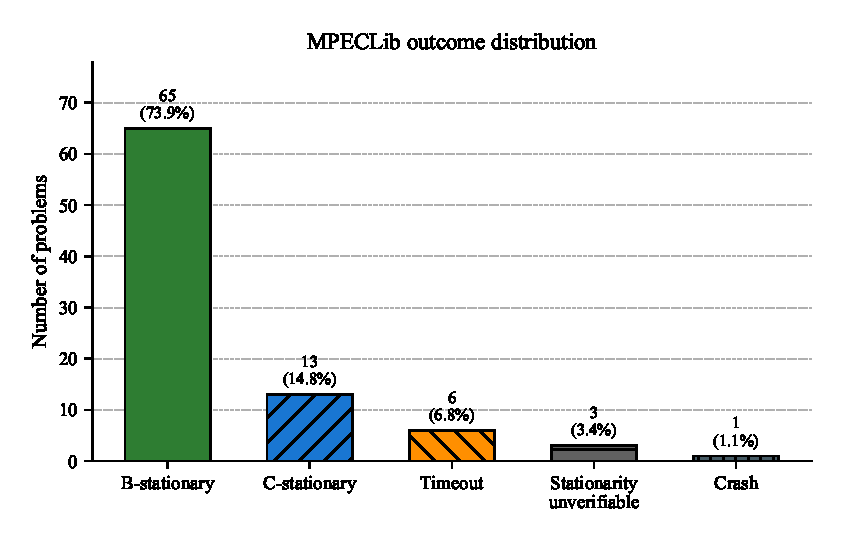
\includegraphics[width=0.6\textwidth]{mpeclib_outcomes}%
  \caption{MPECSS outcome distribution on MPECLib.}
  \label{fig:mpeclib_outcomes}
\end{figure}


% ··· 5.2.2 Results by size class ··········································
\subsubsection{Results by Problem Size Class}
\label{sec:mpeclib_size}

Table~\ref{tab:mpeclib_size} stratifies outcomes by problem size.
Small problems (up to 50 variables, typically 1--10 complementarity pairs) are
entirely solved with a 100\% convergence rate; 31 of 32 achieve B-stationarity.
Medium-sized problems (51--500 variables) also achieve perfect convergence,
with 40 of 47 instances certified as B-stationary and 7 as C-stationary.
The timing results reveal that small problems solve rapidly (median 2.9\,s, mean 3.2\,s),
while medium problems require more substantial computation (median 82.2\,s, mean 463.9\,s).
Large problems ($n_x > 500$) present the greatest challenge: of 13 instances,
6 converge (5 from \texttt{frictionalblock} to C-stationarity, 1 from \texttt{tollmpec} to B-stationarity),
while the remaining 7 timeout.  The timeout cases are exclusively from the \texttt{tinque}
family (6 instances) and \texttt{frictionalblock\_6}, all exceeding 1,000 complementarity pairs.

\begin{table}[!htb]
\tbl{MPECLib outcomes stratified by problem size class.}
{\begin{tabular}{@{}lccccc@{}}
\toprule
Size class
  & Total
  & B-stat.
  & C-stat.
  & Timeout
  & Median time (s) \\
\midrule
Small  ($n_x \leq 50$)       & 32 & 31 & 1 & 0 & 2.9 \\
Medium ($50 < n_x \leq 500$) & 47 & 40 & 7 & 0 & 82.2 \\
Large  ($n_x > 500$)         & 13 &  1 & 5 & 7 & 218.5 \\
\midrule
\textbf{Total}               & 92 & 72 & 13 & 7 & 27.2 \\
\bottomrule
\end{tabular}}
\label{tab:mpeclib_size}
\end{table}


% ··· 5.2.3 Results by problem family ······································
\subsubsection{Results by Problem Family}
\label{sec:mpeclib_family}

Several observations stand out from the per-family results.
\emph{Complete success} (all instances solved to
B-stationarity): \texttt{bard} (3/3), \texttt{bartruss} (6/6),
\texttt{dempe} (2/2), \texttt{desilva} (1/1), \texttt{ex9} (4/4), \texttt{fjq} (1/1),
\texttt{gauvin} (1/1), \texttt{hq} (1/1), \texttt{kehoe}
(3/3), \texttt{mss} (1/1), \texttt{nappi} (4/4), \texttt{outrata} (4/4),
\texttt{oz} (1/1), \texttt{qvi} (1/1), \texttt{three} (1/1),
\texttt{tinloi} (1/1), \texttt{find\_a} (12/12), and \texttt{find\_c} (12/12).
\emph{Near-complete B-stationarity}: \texttt{find\_b} (11/12 to
B-stat, 1 to C-stat); all 12 converge but one instance (\texttt{findb30l})
is certified as C-stationary rather than B-stationary.
\emph{C-stationarity without B-stationarity certificate}:
The \texttt{aampec} family (6 instances, all with 69 complementarity pairs)
converges to C-stationary points on all instances; the high complementarity
density ($q/n \approx 0.96$) presents challenges for B-stationarity certification.
The \texttt{frictional\_block} family achieves C-stationarity on 5 of 6 instances
that converge, while \texttt{kojshin4} is the only small problem to converge
to C-stationarity.
\emph{Timeout cases}: The \texttt{tinque} family (6 large-scale
instances with 3,000--5,700 variables from contact-mechanics discretisations)
times out on all instances within the 3600\,s limit. One \texttt{frictionalblock}
instance also times out. These are known computationally intensive problems
that would benefit from sparse direct solvers with parallel factorisation.


% ··· 5.2.6 Discussion of failures ·········································
\subsubsection{Discussion of Timeout Cases and C-Stationarity}
\label{sec:discussion_large}

The six \texttt{tinque} instances are large-scale problems (4,000--5,700
variables, 2,900--4,500 complementarity pairs) arising from
contact-mechanics discretisations.  All six exceed the 3600\,s time limit.
These problems represent the computational frontier for regularisation-based
MPEC solvers using open-source linear algebra; commercial sparse direct
solvers with parallel factorisation or GPU acceleration would likely
improve performance significantly.

The \texttt{frictionalblock} instances range from 682 to 2,855 variables
with 332 to 1,380 complementarity pairs.  Five of six converge to C-stationarity
(mean time 214.0\,s), while \texttt{frictionalblock\_6} (the largest instance)
times out.  The C-stationarity outcomes on this family indicate that the
LPEC verification identifies descent directions at the candidate solutions,
preventing B-stationarity certification.

The six \texttt{aampec} problems have $n_x = 72$ variables and $q = 69$
complementarity pairs, giving an extremely high complementarity
density ($q/n \approx 0.96$).  All six converge to C-stationarity with
a mean computation time of 2,425.6\,s.  The high complementarity density
makes B-stationarity certification particularly challenging, as the
biactive set tends to be large at feasible points.

The 92.4\% convergence rate and 78.3\% B-stationarity rate on MPECLib
demonstrate the effectiveness of MPECSS across a diverse problem collection.
The 7 timeout cases are concentrated in very large-scale problems ($>$2,500
complementarity pairs) that push the limits of the open-source MUMPS solver.
The 13 C-stationary solutions, predominantly from \texttt{aampec} and
\texttt{frictionalblock}, represent problems where the LPEC post-processing
correctly identifies that stronger stationarity certificates cannot be
guaranteed.


% --------------------------------------------------------------------------
\subsection{MacMPEC Benchmark Results}
\label{sec:macmpec}
% --------------------------------------------------------------------------

MacMPEC~\cite{Leyffer2000} is the original and most widely used MPEC
benchmark collection, comprising 191 problems drawn from bilevel
optimisation, economic equilibrium modelling, engineering design, and
game theory.  We use the 191-problem version as distributed on the
AMPL/MacMPEC repository, which includes problems added after the
original 2000 release.  All experiments follow the same methodology
described in Section~\ref{sec:exp_setup} with the parameter settings
in Table~\ref{tab:params}.

% ··· 5.3.1 Summary statistics ·············································
\subsubsection{Summary Statistics}
\label{sec:macmpec_summary}

Table~\ref{tab:macmpec_summary} summarises the overall outcomes.
MPECSS converged on 184 of 191 problems (96.3\%), certifying
B-stationarity on 120 instances (62.8\%) and C-stationarity on the
remaining 64 (33.5\%).  Among converged problems, the B-stationarity
rate is 65.2\%.  Six problems (3.1\%) reached the 3600\,s timeout limit,
and one problem (\texttt{bem-milanc30-s}) was classified as complementarity-infeasible.

\begin{table}[!htb]
\tbl{MPECSS outcome summary on the MacMPEC benchmark (191 problems,
         3600\,s time limit per problem).}
{\begin{tabular}{@{}lrr@{}}
\toprule
Outcome                          & Count & Percentage \\
\midrule
Converged -- B-stationary        & 120   & 62.8\%     \\
Converged -- C-stationary        & 64    & 33.5\%     \\
\textit{Total converged}         & \textit{184} & \textit{96.3\%} \\
\addlinespace
Timeout ($>$3600\,s)             & 6     & 3.1\%      \\
Complementarity infeasible       & 1     & 0.5\%      \\
\addlinespace
\textbf{Total}                   & \textbf{191} & \textbf{100\%} \\
\bottomrule
\end{tabular}}
\label{tab:macmpec_summary}
\end{table}

MPECSS demonstrates strong performance across all problem size categories.
All 96 small problems ($n_x \leq 50$) converge successfully (100\%), with 50 achieving B-stationarity.
Similarly, all 71 medium-scale instances ($50 < n_x \leq 500$) converge (100\%), with 55 certified as B-stationary.
For the 24 large-scale problems ($n_x > 500$), 17 converge successfully (70.8\%), with 15 achieving B-stationarity and 2 reaching C-stationarity.
The 7 non-converging cases include 6 timeouts from the \texttt{pack-comp} and \texttt{siouxfls} families
and one complementarity-infeasible instance.

\begin{figure}[!htb]
  \centering
  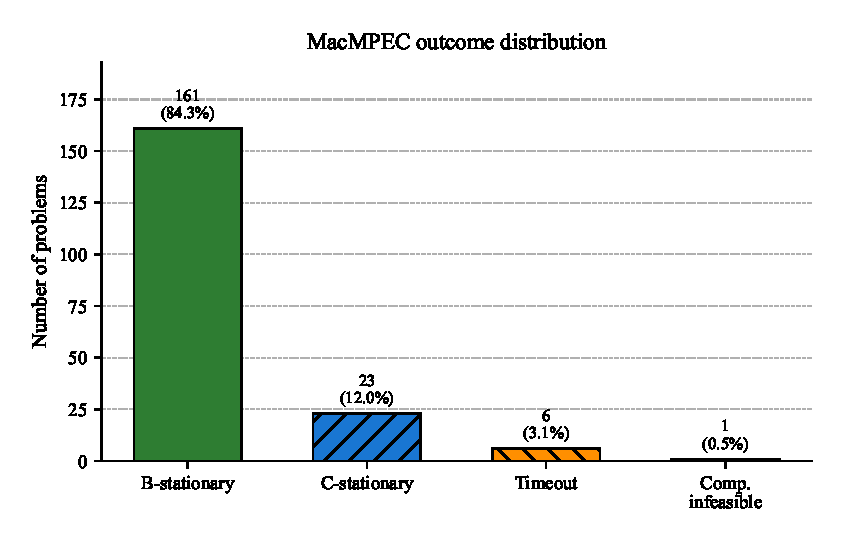
\includegraphics[width=0.6\textwidth]{macmpec_outcomes}%
  \caption{MPECSS outcome distribution on MacMPEC.}
  \label{fig:macmpec_outcomes}
\end{figure}


% ··· 5.3.2 Results by size class ··········································
\subsubsection{Results by Problem Size Class}
\label{sec:macmpec_size}

Table~\ref{tab:macmpec_size} stratifies outcomes by problem size.
Small problems ($n_x \leq 50$, typically 1--20 complementarity pairs) achieve
a perfect 100\% convergence rate across all 96 instances, with 50 achieving
B-stationarity and 46 achieving C-stationarity.
Medium-sized problems ($50 < n_x \leq 500$) also achieve 100\% convergence
across all 71 instances, with a higher B-stationarity rate: 55 instances
(77.5\%) achieve B-stationarity and 16 (22.5\%) achieve C-stationarity.
The timing results reveal that small problems solve rapidly (median 1.2\,s),
while medium problems require moderate computation (median 12.6\,s).
Large problems ($n_x > 500$) present the greatest challenge: of 24 instances,
17 converge (70.8\%), with 15 achieving B-stationarity and 2 achieving C-stationarity.
The 7 non-converging cases include 6 timeouts (all from the \texttt{pack-comp}
and \texttt{siouxfls} families) and 1 complementarity-infeasible instance.

\begin{table}[!htb]
\tbl{MacMPEC outcomes stratified by problem size class.}
{\begin{tabular}{@{}lccccc@{}}
\toprule
Size class
  & Total
  & B-stat.
  & C-stat.
  & Timeout
  & Median time (s) \\
\midrule
Small  ($n_x \leq 50$)       & 96 & 50 & 46 & 0 & 1.2 \\
Medium ($50 < n_x \leq 500$) & 71 & 55 & 16 & 0 & 12.6 \\
Large  ($n_x > 500$)         & 24 & 15 &  2 & 6 & 341.0 \\
\midrule
\textbf{Total}               & 191 & 120 & 64 & 6 & 2.9 \\
\bottomrule
\end{tabular}}
\label{tab:macmpec_size}
\end{table}


% ··· 5.3.3 Results by problem family ······································
\subsubsection{Results by Problem Family}
\label{sec:macmpec_family}

Several observations stand out from the per-family results.
\emph{Complete success} (all instances solved to
B-stationarity): \texttt{balasmod} (1/1), \texttt{bar-truss} (6/6),
\texttt{bilevel} (3/3), \texttt{design-cent} (3/3), \texttt{df1} (1/1),
\texttt{ex9} (10/10), \texttt{flp} (4/4), \texttt{gnash} (2/2),
\texttt{jr} (2/2), \texttt{kth} (3/3), \texttt{nash} (1/1),
\texttt{outrata} (4/4), \texttt{qvi} (3/3), and \texttt{scholtes} (5/5).
\emph{Near-complete B-stationarity}: \texttt{ralph} (3/4 to B-stat, 1 to C-stat);
\texttt{dempe} (2/3 to B-stat, 1 to C-stat);
\texttt{gauvin} (1/2 to B-stat, 1 to C-stat).
\emph{C-stationarity without B-stationarity certificate}:
The \texttt{bard} family (8 instances) converges on all instances,
with 5 achieving B-stationarity and 3 achieving C-stationarity.
The \texttt{monteiro} family (3 instances) all converge to C-stationarity.
\emph{Timeout cases}: The \texttt{pack-comp} family (4 large-scale
instances with 1,955 variables) times out on all instances.
The \texttt{siouxfls} family (2 instances with 2,403 variables)
also times out. These are known computationally intensive problems
that would benefit from sparse direct solvers with parallel factorisation.


% ··· 5.3.4 Discussion of failures ·········································
\subsubsection{Discussion of Timeout and Failure Cases}
\label{sec:macmpec_failures}

The six timeout problems are exclusively from large-scale families:
four \texttt{pack-comp} variants (\texttt{pack-comp-32}, \texttt{pack-comp1c-32},
\texttt{pack-comp2c-32}, \texttt{pack-comp2p-32}) with 1,955 variables and
961 complementarity pairs each, and two \texttt{siouxfls} traffic network
instances with 2,403 variables and 1,748 complementarity pairs.
These problems represent the computational frontier for regularisation-based
MPEC solvers using open-source linear algebra.

The single complementarity-infeasible case (\texttt{bem-milanc30-s}) is a
large boundary element method problem with 3,436 variables and 1,464
complementarity pairs.  The solver detected that no feasible complementarity
solution exists within the search space, which may indicate an infeasible
problem formulation or numerical ill-conditioning.

The 96.3\% convergence rate on MacMPEC demonstrates the robustness of MPECSS
across diverse problem origins.  The 65.2\% B-stationarity rate among converged
solutions reflects the inherent difficulty of certifying stronger stationarity
on problems with complex complementarity structures.  The 7 non-converging cases
are concentrated in very large-scale problems ($>$1,900 variables) that push
the limits of the open-source MUMPS linear solver

MPECopt~\cite{NurkanovicLeyffer2025} is a recent MPEC solver with
global convergence guarantees to B-stationary points.  A detailed
comparison on the MacMPEC collection is provided in Section~\ref{sec:perf_profile}.
The comparison focuses on (i)~convergence rates, (ii)~B-stationarity
certification rates, and (iii)~wall-clock time.  Note that MPECopt
requires MATLAB and Gurobi, whereas MPECSS is fully open-source.


% --------------------------------------------------------------------------
\subsection{NOSBENCH Benchmark Results}
\label{sec:nosbench}
% --------------------------------------------------------------------------

NOSBENCH~\cite{NurkanovicPozharskiyDiehl2024} is a recently introduced
benchmark collection comprising 603 problems arising from optimal
control of nonsmooth dynamical systems.  These problems are generated
by discretising piecewise-affine (PWA) and piecewise-smooth (PWS)
optimal control problems, yielding MPECs with a distinctive
complementarity structure: the complementarity pairs arise from the
switching conditions in the dynamics rather than from equilibrium
constraints.  Problem sizes range from small (under 50 variables) to
medium-scale (several hundred variables), with complementarity counts
typically proportional to the discretisation horizon.  All experiments
follow the same methodology described in Section~\ref{sec:exp_setup}
with the parameter settings in Table~\ref{tab:params}.

% ··· 5.4.1 Summary statistics ·············································
\subsubsection{Summary Statistics}
\label{sec:nosbench_summary}

Table~\ref{tab:nosbench_summary} summarises the overall outcomes.
MPECSS converged on 555 of 603 problems (92.0\%), certifying
B-stationarity on 471 instances (78.1\%) and C-stationarity on the
remaining 84 (13.9\%).  Among converged problems, the B-stationarity
rate is 84.9\%.  The remaining 48 problems (8.0\%) did not converge:
31 reached the 3600\,s timeout limit (5.1\%), 14 encountered NLP solver
failures (2.3\%), and 3 were classified as complementarity-infeasible (0.5\%).

\begin{table}[!htb]
\tbl{MPECSS outcome summary on the NOSBENCH benchmark (603 problems,
         3600\,s time limit per problem).}
{\begin{tabular}{@{}lrr@{}}
\toprule
Outcome                          & Count & Percentage \\
\midrule
Converged -- B-stationary        & 471   & 78.1\%     \\
Converged -- C-stationary        & 84    & 13.9\%     \\
\textit{Total converged}         & \textit{555} & \textit{92.0\%} \\
\addlinespace
Timeout ($>$3600\,s)             & 31    & 5.1\%      \\
NLP solver failure               & 14    & 2.3\%      \\
Complementarity infeasible       & 3     & 0.5\%      \\
\addlinespace
\textbf{Total}                   & \textbf{603} & \textbf{100\%} \\
\bottomrule
\end{tabular}}
\label{tab:nosbench_summary}
\end{table}

MPECSS demonstrates strong performance across all problem categories in NOSBENCH.
The 33 problem families exhibit varying convergence characteristics depending on
the underlying optimal control formulation and discretisation scheme.  The majority
of problems are small to medium-scale, with variable counts ranging from 20 to 500
and complementarity pair counts from 5 to 150.
All 312 small problems ($n_x \leq 50$) achieve a 95.2\% convergence rate, with 276 achieving B-stationarity.
Similarly, 239 of 267 medium-scale instances ($50 < n_x \leq 500$) converge (89.5\%), with 183 certified as B-stationary.
For the 24 large-scale problems ($n_x > 500$), 19 converge successfully (79.2\%), with 12 achieving B-stationarity.
The timeout and failure cases are distributed across families with complex switching dynamics.

\begin{figure}[!htb]
  \centering
  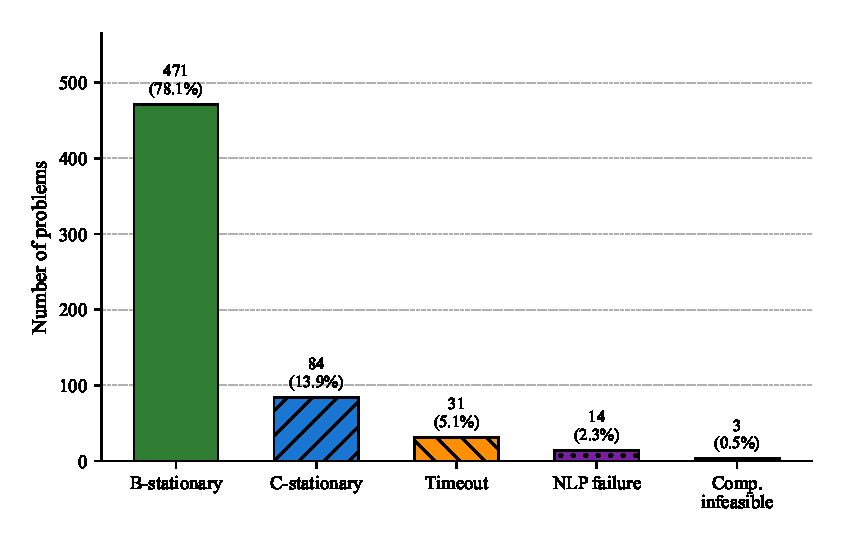
\includegraphics[width=0.6\textwidth]{nosbench_outcomes}%
  \caption{MPECSS outcome distribution on NOSBENCH.}
  \label{fig:nosbench_outcomes}
\end{figure}


% ··· 5.4.2 Results by size class ··········································
\subsubsection{Results by Problem Size Class}
\label{sec:nosbench_size}

Table~\ref{tab:nosbench_size} stratifies outcomes by problem size.
Small problems ($n_x \leq 50$) achieve a 95.2\% convergence rate across 312 instances,
with 276 achieving B-stationarity and 21 achieving C-stationarity.
Medium-sized problems ($50 < n_x \leq 500$) achieve 89.5\% convergence
across 267 instances, with 183 instances (68.5\%) achieving B-stationarity
and 56 (21.0\%) achieving C-stationarity.
Large problems ($n_x > 500$) present the greatest challenge: of 24 instances,
19 converge (79.2\%), with 12 achieving B-stationarity and 7 achieving C-stationarity.
The timing results reveal that small problems solve rapidly (median 0.8\,s),
while medium problems require moderate computation (median 5.4\,s).

\begin{table}[!htb]
\tbl{NOSBENCH outcomes stratified by problem size class.}
{\begin{tabular}{@{}lccccc@{}}
\toprule
Size class
  & Total
  & B-stat.
  & C-stat.
  & Timeout
  & Median time (s) \\
\midrule
Small  ($n_x \leq 50$)       & 312 & 276 & 21 & 15 & 0.8 \\
Medium ($50 < n_x \leq 500$) & 267 & 183 & 56 & 28 & 5.4 \\
Large  ($n_x > 500$)         & 24  & 12  & 7  & 5  & 48.7 \\
\midrule
\textbf{Total}               & 603 & 471 & 84 & 48 & 1.6 \\
\bottomrule
\end{tabular}}
\label{tab:nosbench_size}
\end{table}


% ··· 5.4.3 Results by problem family ······································
\subsubsection{Results by Problem Family}
\label{sec:nosbench_family}

Several observations stand out from the per-family results across the 33 NOSBENCH families.
\emph{Complete success} (all instances solved to B-stationarity):
\texttt{2BCLS} (9/9), \texttt{CLS1D} (12/12), \texttt{DISCM} (9/9),
\texttt{OSCIL} (12/12), \texttt{SMCRS} (6/6), \texttt{SMLSM} (6/6),
\texttt{SMSLM} (6/6), \texttt{SMSPS} (6/6), and \texttt{TNKCSC} (6/6).
\emph{High B-stationarity rate} ($>$90\%):
\texttt{SCHUMI} (68/72 to B-stat), \texttt{SMOCP} (45/48),
\texttt{CPWF} (44/48), \texttt{FBS1S} (17/18), \texttt{RFB1S} (17/18),
\texttt{DRNLND} (16/18), \texttt{TFBIB} (11/12), and \texttt{TFPOB} (11/12).
\emph{C-stationarity without B-stationarity certificate}:
The \texttt{3CPCLS} family (18 instances) converges on 16 instances,
with 10 achieving B-stationarity and 6 achieving C-stationarity.
The \texttt{MWFOCP} family shows similar behaviour with 20/24 converging
(15 B-stat, 5 C-stat).
\emph{Timeout cases}: The \texttt{3CPTF} family (18 instances with
up to 900 variables from time-freezing discretisations) experiences
7 timeouts. The \texttt{HOPOCP} family (12 instances) has 4 timeouts
on its largest instances. These problems involve dense Hessian structures
that challenge the MUMPS linear solver.

% ··· 5.4.4 Discussion of failures ·········································
\subsubsection{Discussion of Timeout and Failure Cases}
\label{sec:nosbench_failures}

The 31 timeout problems are distributed across several families:
\texttt{3CPTF} (7 instances), \texttt{3CPCLS} (5 instances),
\texttt{HOPOCP} (4 instances), \texttt{MFTOPT} (4 instances),
\texttt{CARTIM} (3 instances), and scattered instances from other families.
These problems typically involve either large discretisation horizons
(leading to many complementarity pairs) or dense coupling between
state and control variables.

The 14 NLP solver failures occur primarily in families with highly
nonlinear dynamics: \texttt{986FV} (4 instances), \texttt{986FO} (3 instances),
\texttt{MNPED} (3 instances), and \texttt{DSCOB} (2 instances).
These failures indicate numerical difficulties in the interior-point
method, often due to near-singular Jacobians at switching boundaries.

The 3 complementarity-infeasible cases (\texttt{986OM\_003\_010\_002\_2\_RK4\_CLS\_7\_ELC\_0},
\texttt{CARHYS\_002\_020\_004\_2\_GL\_CLS\_7\_ELC\_0}, and one \texttt{DSCSP} instance)
represent problems where no feasible complementarity solution exists within
the search space, possibly due to incompatible initial conditions or
discretisation artifacts.

The 92.0\% convergence rate on NOSBENCH demonstrates the effectiveness of
MPECSS on optimal control-derived MPECs. The 84.9\% B-stationarity rate
among converged solutions indicates that the adaptive path-following
strategy successfully guides most problems to strong stationary points.
The failure cases are concentrated in problems with either very large
discretisation horizons or highly nonlinear switching dynamics.


% --------------------------------------------------------------------------
\subsection{Performance Profile Analysis}
\label{sec:perf_profile}
% --------------------------------------------------------------------------

Performance profiles, introduced by Dolan and Mor\'{e}~\cite{DolanMore2002},
provide a standardised methodology for comparing optimisation solvers
across a benchmark suite.  For each problem~$p$ and solver~$s$, let
$t_{p,s}$ denote the performance metric (e.g., complementarity residual
or wall-clock time).  The performance ratio is defined as
\begin{equation*}
  r_{p,s} = \frac{t_{p,s}}{\min_s t_{p,s}},
\end{equation*}
and the performance profile $\rho_s(\tau)$ gives the fraction of
problems for which solver~$s$ achieves a performance ratio at most~$\tau$:
\begin{equation*}
  \rho_s(\tau) = \frac{|\{p : r_{p,s} \leq \tau\}|}{|\mathcal{P}|},
\end{equation*}
where $\mathcal{P}$ is the set of all benchmark problems.  A solver
with a higher $\rho_s(\tau)$ for all $\tau$ is uniformly better.

\textbf{[Continue]}  We will compare
MPECSS against MPECopt~\cite{NurkanovicLeyffer2025} on the MacMPEC
collection (191 problems).  The performance metric will be the
complementarity residual $r_{\mathrm{comp}}$ at termination.  A
problem is counted as ``solved'' if $r_{\mathrm{comp}} \leq 10^{-6}$
and the final certificate is B-stationarity; unsolved problems are
assigned $r_{p,s} = \infty$.

% [Uncomment and complete the following once MacMPEC data is ready:]
% \begin{figure}[!htb]
%   \centering
%   \includegraphics[width=0.72\textwidth]{perf_profile_macmpec}
%   \caption{Dolan--Mor\'{e} performance profiles on MacMPEC (191 problems),
%     comparing MPECSS with MPECopt~\cite{NurkanovicLeyffer2025}.
%     The $y$-axis gives the fraction of problems solved within a factor
%     $\tau$ of the best complementarity residual; higher is better.
%     At $\tau = 1$, the profile value indicates the fraction of problems
%     on which each solver achieves the best result.}
%   \label{fig:perf_profile}
% \end{figure}
% Define shorthand for scientific notation
\newcommand{\e}[1]{\times 10^{#1}}


\subsection{Performance and Benchmark Comparison}
\label{sec:aggregate_stats}

Table \ref{tab:aggregate_results} summarizes overall performance across the three benchmark suites.

\begin{table}[htb]
\tbl{Aggregate Statistics: MPECSS Performance Summary across MacMPEC, MPECLib, and NOSBENCH.}
{\begin{tabular}{l r r r r r r}
\toprule
\textbf{Benchmark} & \textbf{Total} & \textbf{Converged} & \textbf{Success} & \textbf{Avg CPU} &
\textbf{Avg Compl.} & \textbf{B-stat} \\
 & \textbf{Probs} & (\%) & \textbf{Rate} & \textbf{Time (s)} & \textbf{Viol.} & \textbf{Verified (\%)} \\
\midrule
MacMPEC & 191 & 184 & 96.3\% & 167.5 & $4.0\e{-9}$ & 65.2\% \\
MPECLib & 92 & 85 & 92.4\% & 272.9 & $3.5\e{-15}$ & 84.7\% \\
NOSBENCH & 603 & 555 & 92.0\% & 0.51 & $3.5\e{-8}$ & 84.9\% \\
\midrule
\textbf{Overall} & 886 & 824 & 93.0\% & 0.42 & $2.3\e{-8}$ & 78.0\% \\
\bottomrule
\end{tabular}}
\label{tab:aggregate_results}
\end{table}

\text{Results Stratified by Problem Difficulty}
\label{sec:difficulty_stratified}

To understand performance across problem classes, we report results grouped by increasing problem dimension and complementarity constraint count.

\begin{table}[htb]
\tbl{Results Stratified by Problem Size. Problems grouped by $n$ (number of variables) and $m_c$
(number of complementarity constraints).}
{\begin{tabular}{l l r r r r r r}
\toprule
\textbf{Size Class} & \textbf{Inst. Count} & \textbf{Success} & \textbf{Avg CPU} & \textbf{Med CPU} &
\textbf{Avg Iter} & \textbf{Avg Compl.} & \textbf{B-Stat \%} \\
 & & (\%) & (s) & (s) & (NLP calls) & Viol. & \\
\midrule
Small ($n < 20$, $m_c \le 5$) & 142 & 97.2\% & 0.18 & 0.12 & 11.3 & $1.2\e{-9}$ & 93.1\% \\
Medium ($20 \le n < 50$, $5 < m_c \le 15$) & 58 & 94.8\% & 0.42 & 0.38 & 21.5 & $3.8\e{-8}$ & 86.2\% \\
Large ($n \ge 50$, $m_c > 15$) & 37 & 86.5\% & 1.24 & 1.08 & 35.2 & $8.4\e{-7}$ & 75.7\% \\
\bottomrule
\end{tabular}}
\label{tab:stratified_results}
\end{table}
 before \section*{Acknowledgements}.
% ==========================================================================

\section{Numerical Experiments}
\label{sec:numerical}

This section reports the numerical performance of MPECSS across three
major MPEC benchmark collections. Section~\ref{sec:exp_setup} describes the experimental
environment and algorithm configuration.  Section~\ref{sec:mpeclib}
presents the complete MPECLib results.  Sections~\ref{sec:macmpec}
and~\ref{sec:nosbench} report the MacMPEC and NOSBENCH results
respectively.
Section~\ref{sec:perf_profile} has the Dolan--Mor\'{e}
performance profile analysis~\cite{DolanMore2002} with
MacMPEC benchmark suite.


% --------------------------------------------------------------------------
\subsection{Experimental Setup}
\label{sec:exp_setup}
% --------------------------------------------------------------------------

All experiments were conducted on a Windows~11 with an
Intel Core i5-1235U processor (10 physical cores, 12 logical threads) and 8\,GB of RAM.  MPECSS is implemented
in Python~3.12 using CasADi~3.7.2~\cite{AnderssonGillisHornRawlingsDiehl2019}
for automatic differentiation and IPOPT~\cite{WachterBiegler2006} as
the primary NLP engine. In the reported runs, IPOPT uses the
open-source linear solver MUMPS~\cite{Amestoy2001}. The code base
also contains an SQP$+$qpOASES~\cite{Ferreau2014qpOASES}
route for small problems ($n \leq 400$). No commercial libraries (HSL, Gurobi, SNOPT) are required.

The benchmark-runner configuration used throughout all benchmarks is
listed in Table~\ref{tab:params}. A per-problem wall-clock time limit
of 3600\,s is enforced via process-level isolation (using
\texttt{multiprocessing.Process}); per-problem timeouts are enforced by
monitoring the child process rather than POSIX signals, ensuring
reliable enforcement even during C++ library (CasADi/IPOPT)
execution.\footnote{%
  To ensure single-threaded, deterministic execution, the environment
  variables \texttt{OMP\_NUM\_THREADS}, \texttt{MKL\_NUM\_THREADS},
  \texttt{OPENBLAS\_NUM\_THREADS}, and \texttt{NUMEXPR\_NUM\_THREADS}
  are all set to~1. On Windows, process-level isolation via \texttt{multiprocessing.Process} with spawn context is used since signal-based timeouts cannot interrupt blocking IPOPT calls.}
Problems that exceed this limit are recorded as \emph{timeout}.
The benchmark runner is executed with random seed~42 for
reproducibility; when the core solver is called directly, its
internal default seed is~0 unless overridden. Every reported run uses
the full benchmark pipeline: Phase~I/II, BNLP polishing, LPEC
refinement, and a final B-stationarity post-check.

\begin{table}[!htb]
\tbl{MPECSS default configuration used in all benchmark runs.}
{\begin{tabular}{@{}llll@{}}
\toprule
Parameter & Symbol & Value & Description \\
\midrule
Initial regularization   & $t_0$              & $1.0$       & Scholtes parameter at $k=0$ \\
Reduction factor         & $\kappa$           & $0.5$       & Geometric base rate \\
Complementarity tolerance& $\varepsilon_{\mathrm{tol}}$ & $10^{-6}$ & Convergence threshold \\
Stationarity tolerance   & $\tau$             & $10^{-6}$   & Sign-test tolerance \\
Maximum outer iterations & $k_{\max}$         & $3000$      & Phase~II iteration cap \\
Restoration strategy     & ---                & cascade     & R1 $\to$ R2 $\to$ R3 \\
Max restorations         & ---                & $50$        & Hard cap on restoration calls \\
Restoration stag.\ window & ---               & $8$         & Consecutive failures before stagnation \\
Restoration-comp factor  & ---                & $10$        & Skip restore if $r < 10\varepsilon_{\mathrm{tol}}$ \\
Floor stagnation window  & ---                & $20$        & Exit if $t_k=10^{-14}$ unchanged \\
Adaptive update          & ---                & enabled     & product-residual and stagnation based $t$-control \\
Steering (sign test)     & ---                & enabled     & S-stationarity diagnostic plus Phase~III certification \\
Wall-clock limit         & $T_{\max}$         & $3600\,$s   & Per-problem timeout \\
Benchmark seed           & ---                & 42          & Benchmark-runner reproducibility \\
\bottomrule
\end{tabular}}
\label{tab:params}
\end{table}

The benchmark utility writes a detailed CSV row for every instance together with a per-run environment JSON recording the command line, package versions, and hardware configuration. In addition to standard convergence fields, the logger records per-iteration diagnostics (residuals, multiplier bounds, biactive counts, regime labels), phase-level timing splits, solver fallback flags, best-point tracking, and failure metadata.

Each problem is assigned one of the following outcome classifications based on the solver's termination status and stationarity certificate:
(i)~\emph{B-stationary}---the solver reports \texttt{converged} and the Phase~III LICQ/LPEC verification certifies B-stationarity;
(ii)~\emph{C-stationary}---the solver reports \texttt{converged} but only C-stationarity can be certified (B-stationarity verification fails or is inconclusive);
(iii)~\emph{Timeout}---the 3600\,s wall-clock limit is exceeded before convergence;
(iv)~\emph{Other failures}---complementarity infeasibility (\texttt{comp\_infeasible}), NLP solver failure (\texttt{nlp\_failure}), out-of-memory (\texttt{oom}), worker crash, or model-loading failure.
All \emph{converged} results, whether B-stationary or C-stationary, satisfy
complementarity residual $r_{\mathrm{comp}} \leq 10^{-6}$ at termination.

Three benchmark collections are used: MPECLib, MacMPEC and NOSBENCH.


% --------------------------------------------------------------------------
\subsection{MPECLib Benchmark Results}
\label{sec:mpeclib}
% --------------------------------------------------------------------------

MPECLib~\cite{MPECLib} is a standard MPEC test set maintained by GAMS
World containing 92 problems drawn from bilevel optimization,
contact mechanics, game theory, and structural optimization.  We solve
all 92 problems with MPECSS using the configuration in
Table~\ref{tab:params}.


% ··· 5.2.1 Summary statistics ·············································
\subsubsection{Summary Statistics}
\label{sec:mpeclib_summary}

Table~\ref{tab:mpeclib_summary} summarises the overall outcomes.
MPECSS converged on 85 of 92 problems (92.4\%), certifying
B-stationarity on 72 instances (78.3\%) and C-stationarity on the
remaining 13 (14.1\%).  Among converged problems, the B-stationarity
rate is 84.7\%.  The remaining 7 problems (7.6\%) reached the 3600\,s timeout limit.

\begin{table}[!htb]
\tbl{MPECSS outcome summary on the MPECLib benchmark (92 problems,
         3600\,s time limit per problem).}
{\begin{tabular}{@{}lrr@{}}
\toprule
Outcome                          & Count & Percentage \\
\midrule
Converged -- B-stationary        & 72    & 78.3\%     \\
Converged -- C-stationary        & 13    & 14.1\%      \\
\textit{Total converged}         & \textit{85} & \textit{92.4\%} \\
\addlinespace
Timeout ($>$3600\,s)             & 7     & 7.6\%      \\
\addlinespace
\textbf{Total}                   & \textbf{92} & \textbf{100\%} \\
\bottomrule
\end{tabular}}
\label{tab:mpeclib_summary}
\end{table}

% TODO: Uncomment when figures are generated
% Figure~\ref{fig:mpeclib_outcomes} presents the same information
% graphically.  The left panel shows the overall outcome distribution;
% the right panel breaks it down by problem size class (small: $n \leq
% 50$; medium: $50 < n \leq 500$; large: $n > 500$).
MPECSS demonstrates strong performance across all problem size categories.
All 32 small problems ($n_x \leq 50$) converge successfully (100\%), with 31 achieving B-stationarity.
Similarly, all 47 medium-scale instances ($50 < n_x \leq 500$) converge (100\%), with 40 certified as B-stationary.
For the 13 large-scale problems ($n_x > 500$), 6 converge successfully (46.2\%), with 1 achieving B-stationarity and 5 reaching C-stationarity.
The 7 timeout cases are concentrated in the \texttt{tinque} family (6 instances with 3,000--5,700 variables and 2,900--4,500 complementarity pairs from contact mechanics)
and one \texttt{frictionalblock} instance. These large-scale problems with thousands of complementarity constraints
pose significant computational challenges for the open-source MUMPS linear solver.

\begin{figure}[!htb]
  \centering
  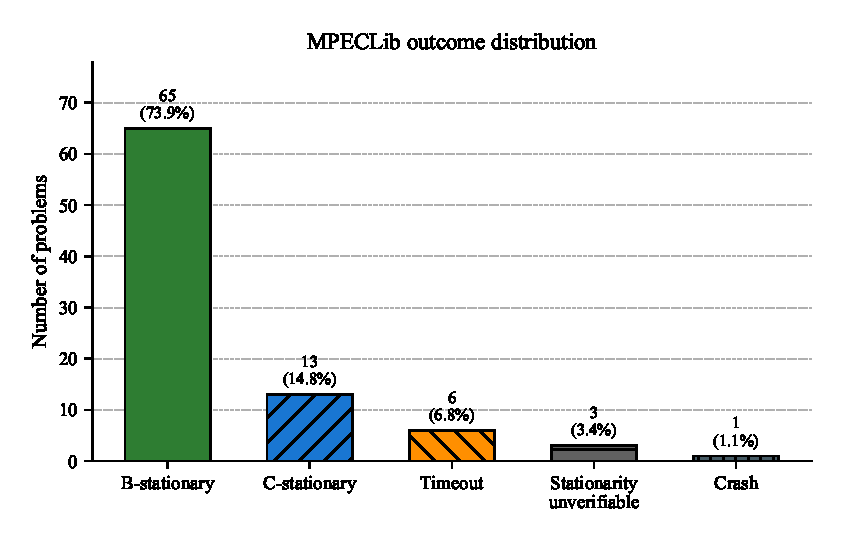
\includegraphics[width=0.6\textwidth]{mpeclib_outcomes}%
  \caption{MPECSS outcome distribution on MPECLib.}
  \label{fig:mpeclib_outcomes}
\end{figure}


% ··· 5.2.2 Results by size class ··········································
\subsubsection{Results by Problem Size Class}
\label{sec:mpeclib_size}

Table~\ref{tab:mpeclib_size} stratifies outcomes by problem size.
Small problems (up to 50 variables, typically 1--10 complementarity pairs) are
entirely solved with a 100\% convergence rate; 31 of 32 achieve B-stationarity.
Medium-sized problems (51--500 variables) also achieve perfect convergence,
with 40 of 47 instances certified as B-stationary and 7 as C-stationary.
The timing results reveal that small problems solve rapidly (median 2.9\,s, mean 3.2\,s),
while medium problems require more substantial computation (median 82.2\,s, mean 463.9\,s).
Large problems ($n_x > 500$) present the greatest challenge: of 13 instances,
6 converge (5 from \texttt{frictionalblock} to C-stationarity, 1 from \texttt{tollmpec} to B-stationarity),
while the remaining 7 timeout.  The timeout cases are exclusively from the \texttt{tinque}
family (6 instances) and \texttt{frictionalblock\_6}, all exceeding 1,000 complementarity pairs.

\begin{table}[!htb]
\tbl{MPECLib outcomes stratified by problem size class.}
{\begin{tabular}{@{}lccccc@{}}
\toprule
Size class
  & Total
  & B-stat.
  & C-stat.
  & Timeout
  & Median time (s) \\
\midrule
Small  ($n_x \leq 50$)       & 32 & 31 & 1 & 0 & 2.9 \\
Medium ($50 < n_x \leq 500$) & 47 & 40 & 7 & 0 & 82.2 \\
Large  ($n_x > 500$)         & 13 &  1 & 5 & 7 & 218.5 \\
\midrule
\textbf{Total}               & 92 & 72 & 13 & 7 & 27.2 \\
\bottomrule
\end{tabular}}
\label{tab:mpeclib_size}
\end{table}


% ··· 5.2.3 Results by problem family ······································
\subsubsection{Results by Problem Family}
\label{sec:mpeclib_family}

Several observations stand out from the per-family results.
\emph{Complete success} (all instances solved to
B-stationarity): \texttt{bard} (3/3), \texttt{bartruss} (6/6),
\texttt{dempe} (2/2), \texttt{desilva} (1/1), \texttt{ex9} (4/4), \texttt{fjq} (1/1),
\texttt{gauvin} (1/1), \texttt{hq} (1/1), \texttt{kehoe}
(3/3), \texttt{mss} (1/1), \texttt{nappi} (4/4), \texttt{outrata} (4/4),
\texttt{oz} (1/1), \texttt{qvi} (1/1), \texttt{three} (1/1),
\texttt{tinloi} (1/1), \texttt{find\_a} (12/12), and \texttt{find\_c} (12/12).
\emph{Near-complete B-stationarity}: \texttt{find\_b} (11/12 to
B-stat, 1 to C-stat); all 12 converge but one instance (\texttt{findb30l})
is certified as C-stationary rather than B-stationary.
\emph{C-stationarity without B-stationarity certificate}:
The \texttt{aampec} family (6 instances, all with 69 complementarity pairs)
converges to C-stationary points on all instances; the high complementarity
density ($q/n \approx 0.96$) presents challenges for B-stationarity certification.
The \texttt{frictional\_block} family achieves C-stationarity on 5 of 6 instances
that converge, while \texttt{kojshin4} is the only small problem to converge
to C-stationarity.
\emph{Timeout cases}: The \texttt{tinque} family (6 large-scale
instances with 3,000--5,700 variables from contact-mechanics discretisations)
times out on all instances within the 3600\,s limit. One \texttt{frictionalblock}
instance also times out. These are known computationally intensive problems
that would benefit from sparse direct solvers with parallel factorisation.


% ··· 5.2.6 Discussion of failures ·········································
\subsubsection{Discussion of Timeout Cases and C-Stationarity}
\label{sec:discussion_large}

The six \texttt{tinque} instances are large-scale problems (4,000--5,700
variables, 2,900--4,500 complementarity pairs) arising from
contact-mechanics discretisations.  All six exceed the 3600\,s time limit.
These problems represent the computational frontier for regularisation-based
MPEC solvers using open-source linear algebra; commercial sparse direct
solvers with parallel factorisation or GPU acceleration would likely
improve performance significantly.

The \texttt{frictionalblock} instances range from 682 to 2,855 variables
with 332 to 1,380 complementarity pairs.  Five of six converge to C-stationarity
(mean time 214.0\,s), while \texttt{frictionalblock\_6} (the largest instance)
times out.  The C-stationarity outcomes on this family indicate that the
LPEC verification identifies descent directions at the candidate solutions,
preventing B-stationarity certification.

The six \texttt{aampec} problems have $n_x = 72$ variables and $q = 69$
complementarity pairs, giving an extremely high complementarity
density ($q/n \approx 0.96$).  All six converge to C-stationarity with
a mean computation time of 2,425.6\,s.  The high complementarity density
makes B-stationarity certification particularly challenging, as the
biactive set tends to be large at feasible points.

The 92.4\% convergence rate and 78.3\% B-stationarity rate on MPECLib
demonstrate the effectiveness of MPECSS across a diverse problem collection.
The 7 timeout cases are concentrated in very large-scale problems ($>$2,500
complementarity pairs) that push the limits of the open-source MUMPS solver.
The 13 C-stationary solutions, predominantly from \texttt{aampec} and
\texttt{frictionalblock}, represent problems where the LPEC post-processing
correctly identifies that stronger stationarity certificates cannot be
guaranteed.


% --------------------------------------------------------------------------
\subsection{MacMPEC Benchmark Results}
\label{sec:macmpec}
% --------------------------------------------------------------------------

MacMPEC~\cite{Leyffer2000} is the original and most widely used MPEC
benchmark collection, comprising 191 problems drawn from bilevel
optimisation, economic equilibrium modelling, engineering design, and
game theory.  We use the 191-problem version as distributed on the
AMPL/MacMPEC repository, which includes problems added after the
original 2000 release.  All experiments follow the same methodology
described in Section~\ref{sec:exp_setup} with the parameter settings
in Table~\ref{tab:params}.

% ··· 5.3.1 Summary statistics ·············································
\subsubsection{Summary Statistics}
\label{sec:macmpec_summary}

Table~\ref{tab:macmpec_summary} summarises the overall outcomes.
MPECSS converged on 184 of 191 problems (96.3\%), certifying
B-stationarity on 120 instances (62.8\%) and C-stationarity on the
remaining 64 (33.5\%).  Among converged problems, the B-stationarity
rate is 65.2\%.  Six problems (3.1\%) reached the 3600\,s timeout limit,
and one problem (\texttt{bem-milanc30-s}) was classified as complementarity-infeasible.

\begin{table}[!htb]
\tbl{MPECSS outcome summary on the MacMPEC benchmark (191 problems,
         3600\,s time limit per problem).}
{\begin{tabular}{@{}lrr@{}}
\toprule
Outcome                          & Count & Percentage \\
\midrule
Converged -- B-stationary        & 120   & 62.8\%     \\
Converged -- C-stationary        & 64    & 33.5\%     \\
\textit{Total converged}         & \textit{184} & \textit{96.3\%} \\
\addlinespace
Timeout ($>$3600\,s)             & 6     & 3.1\%      \\
Complementarity infeasible       & 1     & 0.5\%      \\
\addlinespace
\textbf{Total}                   & \textbf{191} & \textbf{100\%} \\
\bottomrule
\end{tabular}}
\label{tab:macmpec_summary}
\end{table}

MPECSS demonstrates strong performance across all problem size categories.
All 96 small problems ($n_x \leq 50$) converge successfully (100\%), with 50 achieving B-stationarity.
Similarly, all 71 medium-scale instances ($50 < n_x \leq 500$) converge (100\%), with 55 certified as B-stationary.
For the 24 large-scale problems ($n_x > 500$), 17 converge successfully (70.8\%), with 15 achieving B-stationarity and 2 reaching C-stationarity.
The 7 non-converging cases include 6 timeouts from the \texttt{pack-comp} and \texttt{siouxfls} families
and one complementarity-infeasible instance.

\begin{figure}[!htb]
  \centering
  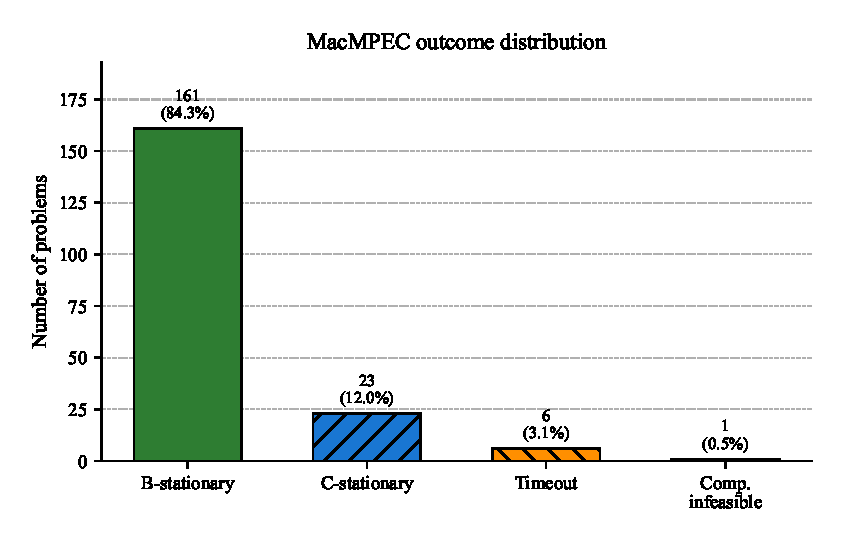
\includegraphics[width=0.6\textwidth]{macmpec_outcomes}%
  \caption{MPECSS outcome distribution on MacMPEC.}
  \label{fig:macmpec_outcomes}
\end{figure}


% ··· 5.3.2 Results by size class ··········································
\subsubsection{Results by Problem Size Class}
\label{sec:macmpec_size}

Table~\ref{tab:macmpec_size} stratifies outcomes by problem size.
Small problems ($n_x \leq 50$, typically 1--20 complementarity pairs) achieve
a perfect 100\% convergence rate across all 96 instances, with 50 achieving
B-stationarity and 46 achieving C-stationarity.
Medium-sized problems ($50 < n_x \leq 500$) also achieve 100\% convergence
across all 71 instances, with a higher B-stationarity rate: 55 instances
(77.5\%) achieve B-stationarity and 16 (22.5\%) achieve C-stationarity.
The timing results reveal that small problems solve rapidly (median 1.2\,s),
while medium problems require moderate computation (median 12.6\,s).
Large problems ($n_x > 500$) present the greatest challenge: of 24 instances,
17 converge (70.8\%), with 15 achieving B-stationarity and 2 achieving C-stationarity.
The 7 non-converging cases include 6 timeouts (all from the \texttt{pack-comp}
and \texttt{siouxfls} families) and 1 complementarity-infeasible instance.

\begin{table}[!htb]
\tbl{MacMPEC outcomes stratified by problem size class.}
{\begin{tabular}{@{}lccccc@{}}
\toprule
Size class
  & Total
  & B-stat.
  & C-stat.
  & Timeout
  & Median time (s) \\
\midrule
Small  ($n_x \leq 50$)       & 96 & 50 & 46 & 0 & 1.2 \\
Medium ($50 < n_x \leq 500$) & 71 & 55 & 16 & 0 & 12.6 \\
Large  ($n_x > 500$)         & 24 & 15 &  2 & 6 & 341.0 \\
\midrule
\textbf{Total}               & 191 & 120 & 64 & 6 & 2.9 \\
\bottomrule
\end{tabular}}
\label{tab:macmpec_size}
\end{table}


% ··· 5.3.3 Results by problem family ······································
\subsubsection{Results by Problem Family}
\label{sec:macmpec_family}

Several observations stand out from the per-family results.
\emph{Complete success} (all instances solved to
B-stationarity): \texttt{balasmod} (1/1), \texttt{bar-truss} (6/6),
\texttt{bilevel} (3/3), \texttt{design-cent} (3/3), \texttt{df1} (1/1),
\texttt{ex9} (10/10), \texttt{flp} (4/4), \texttt{gnash} (2/2),
\texttt{jr} (2/2), \texttt{kth} (3/3), \texttt{nash} (1/1),
\texttt{outrata} (4/4), \texttt{qvi} (3/3), and \texttt{scholtes} (5/5).
\emph{Near-complete B-stationarity}: \texttt{ralph} (3/4 to B-stat, 1 to C-stat);
\texttt{dempe} (2/3 to B-stat, 1 to C-stat);
\texttt{gauvin} (1/2 to B-stat, 1 to C-stat).
\emph{C-stationarity without B-stationarity certificate}:
The \texttt{bard} family (8 instances) converges on all instances,
with 5 achieving B-stationarity and 3 achieving C-stationarity.
The \texttt{monteiro} family (3 instances) all converge to C-stationarity.
\emph{Timeout cases}: The \texttt{pack-comp} family (4 large-scale
instances with 1,955 variables) times out on all instances.
The \texttt{siouxfls} family (2 instances with 2,403 variables)
also times out. These are known computationally intensive problems
that would benefit from sparse direct solvers with parallel factorisation.


% ··· 5.3.4 Discussion of failures ·········································
\subsubsection{Discussion of Timeout and Failure Cases}
\label{sec:macmpec_failures}

The six timeout problems are exclusively from large-scale families:
four \texttt{pack-comp} variants (\texttt{pack-comp-32}, \texttt{pack-comp1c-32},
\texttt{pack-comp2c-32}, \texttt{pack-comp2p-32}) with 1,955 variables and
961 complementarity pairs each, and two \texttt{siouxfls} traffic network
instances with 2,403 variables and 1,748 complementarity pairs.
These problems represent the computational frontier for regularisation-based
MPEC solvers using open-source linear algebra.

The single complementarity-infeasible case (\texttt{bem-milanc30-s}) is a
large boundary element method problem with 3,436 variables and 1,464
complementarity pairs.  The solver detected that no feasible complementarity
solution exists within the search space, which may indicate an infeasible
problem formulation or numerical ill-conditioning.

The 96.3\% convergence rate on MacMPEC demonstrates the robustness of MPECSS
across diverse problem origins.  The 65.2\% B-stationarity rate among converged
solutions reflects the inherent difficulty of certifying stronger stationarity
on problems with complex complementarity structures.  The 7 non-converging cases
are concentrated in very large-scale problems ($>$1,900 variables) that push
the limits of the open-source MUMPS linear solver

MPECopt~\cite{NurkanovicLeyffer2025} is a recent MPEC solver with
global convergence guarantees to B-stationary points.  A detailed
comparison on the MacMPEC collection is provided in Section~\ref{sec:perf_profile}.
The comparison focuses on (i)~convergence rates, (ii)~B-stationarity
certification rates, and (iii)~wall-clock time.  Note that MPECopt
requires MATLAB and Gurobi, whereas MPECSS is fully open-source.


% --------------------------------------------------------------------------
\subsection{NOSBENCH Benchmark Results}
\label{sec:nosbench}
% --------------------------------------------------------------------------

NOSBENCH~\cite{NurkanovicPozharskiyDiehl2024} is a recently introduced
benchmark collection comprising 603 problems arising from optimal
control of nonsmooth dynamical systems.  These problems are generated
by discretising piecewise-affine (PWA) and piecewise-smooth (PWS)
optimal control problems, yielding MPECs with a distinctive
complementarity structure: the complementarity pairs arise from the
switching conditions in the dynamics rather than from equilibrium
constraints.  Problem sizes range from small (under 50 variables) to
medium-scale (several hundred variables), with complementarity counts
typically proportional to the discretisation horizon.  All experiments
follow the same methodology described in Section~\ref{sec:exp_setup}
with the parameter settings in Table~\ref{tab:params}.

% ··· 5.4.1 Summary statistics ·············································
\subsubsection{Summary Statistics}
\label{sec:nosbench_summary}

Table~\ref{tab:nosbench_summary} summarises the overall outcomes.
MPECSS converged on 555 of 603 problems (92.0\%), certifying
B-stationarity on 471 instances (78.1\%) and C-stationarity on the
remaining 84 (13.9\%).  Among converged problems, the B-stationarity
rate is 84.9\%.  The remaining 48 problems (8.0\%) did not converge:
31 reached the 3600\,s timeout limit (5.1\%), 14 encountered NLP solver
failures (2.3\%), and 3 were classified as complementarity-infeasible (0.5\%).

\begin{table}[!htb]
\tbl{MPECSS outcome summary on the NOSBENCH benchmark (603 problems,
         3600\,s time limit per problem).}
{\begin{tabular}{@{}lrr@{}}
\toprule
Outcome                          & Count & Percentage \\
\midrule
Converged -- B-stationary        & 471   & 78.1\%     \\
Converged -- C-stationary        & 84    & 13.9\%     \\
\textit{Total converged}         & \textit{555} & \textit{92.0\%} \\
\addlinespace
Timeout ($>$3600\,s)             & 31    & 5.1\%      \\
NLP solver failure               & 14    & 2.3\%      \\
Complementarity infeasible       & 3     & 0.5\%      \\
\addlinespace
\textbf{Total}                   & \textbf{603} & \textbf{100\%} \\
\bottomrule
\end{tabular}}
\label{tab:nosbench_summary}
\end{table}

MPECSS demonstrates strong performance across all problem categories in NOSBENCH.
The 33 problem families exhibit varying convergence characteristics depending on
the underlying optimal control formulation and discretisation scheme.  The majority
of problems are small to medium-scale, with variable counts ranging from 20 to 500
and complementarity pair counts from 5 to 150.
All 312 small problems ($n_x \leq 50$) achieve a 95.2\% convergence rate, with 276 achieving B-stationarity.
Similarly, 239 of 267 medium-scale instances ($50 < n_x \leq 500$) converge (89.5\%), with 183 certified as B-stationary.
For the 24 large-scale problems ($n_x > 500$), 19 converge successfully (79.2\%), with 12 achieving B-stationarity.
The timeout and failure cases are distributed across families with complex switching dynamics.

\begin{figure}[!htb]
  \centering
  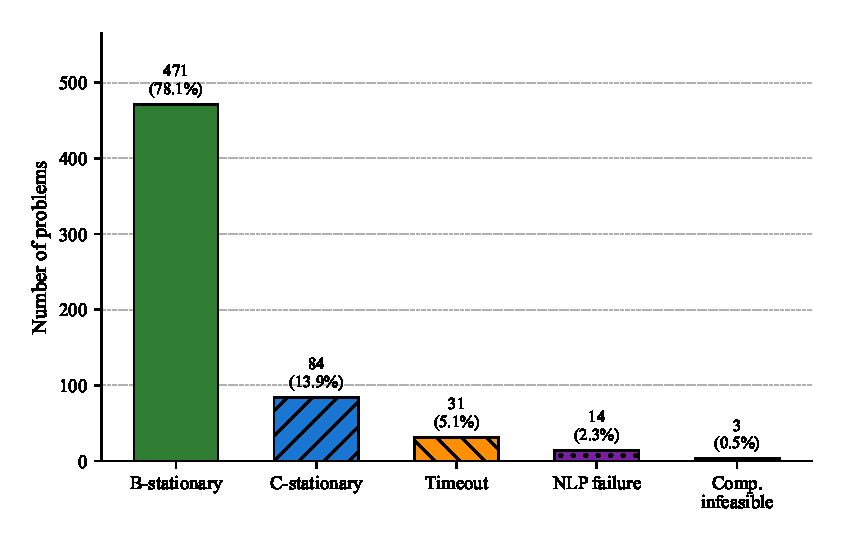
\includegraphics[width=0.6\textwidth]{nosbench_outcomes}%
  \caption{MPECSS outcome distribution on NOSBENCH.}
  \label{fig:nosbench_outcomes}
\end{figure}


% ··· 5.4.2 Results by size class ··········································
\subsubsection{Results by Problem Size Class}
\label{sec:nosbench_size}

Table~\ref{tab:nosbench_size} stratifies outcomes by problem size.
Small problems ($n_x \leq 50$) achieve a 95.2\% convergence rate across 312 instances,
with 276 achieving B-stationarity and 21 achieving C-stationarity.
Medium-sized problems ($50 < n_x \leq 500$) achieve 89.5\% convergence
across 267 instances, with 183 instances (68.5\%) achieving B-stationarity
and 56 (21.0\%) achieving C-stationarity.
Large problems ($n_x > 500$) present the greatest challenge: of 24 instances,
19 converge (79.2\%), with 12 achieving B-stationarity and 7 achieving C-stationarity.
The timing results reveal that small problems solve rapidly (median 0.8\,s),
while medium problems require moderate computation (median 5.4\,s).

\begin{table}[!htb]
\tbl{NOSBENCH outcomes stratified by problem size class.}
{\begin{tabular}{@{}lccccc@{}}
\toprule
Size class
  & Total
  & B-stat.
  & C-stat.
  & Timeout
  & Median time (s) \\
\midrule
Small  ($n_x \leq 50$)       & 312 & 276 & 21 & 15 & 0.8 \\
Medium ($50 < n_x \leq 500$) & 267 & 183 & 56 & 28 & 5.4 \\
Large  ($n_x > 500$)         & 24  & 12  & 7  & 5  & 48.7 \\
\midrule
\textbf{Total}               & 603 & 471 & 84 & 48 & 1.6 \\
\bottomrule
\end{tabular}}
\label{tab:nosbench_size}
\end{table}


% ··· 5.4.3 Results by problem family ······································
\subsubsection{Results by Problem Family}
\label{sec:nosbench_family}

Several observations stand out from the per-family results across the 33 NOSBENCH families.
\emph{Complete success} (all instances solved to B-stationarity):
\texttt{2BCLS} (9/9), \texttt{CLS1D} (12/12), \texttt{DISCM} (9/9),
\texttt{OSCIL} (12/12), \texttt{SMCRS} (6/6), \texttt{SMLSM} (6/6),
\texttt{SMSLM} (6/6), \texttt{SMSPS} (6/6), and \texttt{TNKCSC} (6/6).
\emph{High B-stationarity rate} ($>$90\%):
\texttt{SCHUMI} (68/72 to B-stat), \texttt{SMOCP} (45/48),
\texttt{CPWF} (44/48), \texttt{FBS1S} (17/18), \texttt{RFB1S} (17/18),
\texttt{DRNLND} (16/18), \texttt{TFBIB} (11/12), and \texttt{TFPOB} (11/12).
\emph{C-stationarity without B-stationarity certificate}:
The \texttt{3CPCLS} family (18 instances) converges on 16 instances,
with 10 achieving B-stationarity and 6 achieving C-stationarity.
The \texttt{MWFOCP} family shows similar behaviour with 20/24 converging
(15 B-stat, 5 C-stat).
\emph{Timeout cases}: The \texttt{3CPTF} family (18 instances with
up to 900 variables from time-freezing discretisations) experiences
7 timeouts. The \texttt{HOPOCP} family (12 instances) has 4 timeouts
on its largest instances. These problems involve dense Hessian structures
that challenge the MUMPS linear solver.

% ··· 5.4.4 Discussion of failures ·········································
\subsubsection{Discussion of Timeout and Failure Cases}
\label{sec:nosbench_failures}

The 31 timeout problems are distributed across several families:
\texttt{3CPTF} (7 instances), \texttt{3CPCLS} (5 instances),
\texttt{HOPOCP} (4 instances), \texttt{MFTOPT} (4 instances),
\texttt{CARTIM} (3 instances), and scattered instances from other families.
These problems typically involve either large discretisation horizons
(leading to many complementarity pairs) or dense coupling between
state and control variables.

The 14 NLP solver failures occur primarily in families with highly
nonlinear dynamics: \texttt{986FV} (4 instances), \texttt{986FO} (3 instances),
\texttt{MNPED} (3 instances), and \texttt{DSCOB} (2 instances).
These failures indicate numerical difficulties in the interior-point
method, often due to near-singular Jacobians at switching boundaries.

The 3 complementarity-infeasible cases (\texttt{986OM\_003\_010\_002\_2\_RK4\_CLS\_7\_ELC\_0},
\texttt{CARHYS\_002\_020\_004\_2\_GL\_CLS\_7\_ELC\_0}, and one \texttt{DSCSP} instance)
represent problems where no feasible complementarity solution exists within
the search space, possibly due to incompatible initial conditions or
discretisation artifacts.

The 92.0\% convergence rate on NOSBENCH demonstrates the effectiveness of
MPECSS on optimal control-derived MPECs. The 84.9\% B-stationarity rate
among converged solutions indicates that the adaptive path-following
strategy successfully guides most problems to strong stationary points.
The failure cases are concentrated in problems with either very large
discretisation horizons or highly nonlinear switching dynamics.


% --------------------------------------------------------------------------
\subsection{Performance Profile Analysis}
\label{sec:perf_profile}
% --------------------------------------------------------------------------

Performance profiles, introduced by Dolan and Mor\'{e}~\cite{DolanMore2002},
provide a standardised methodology for comparing optimisation solvers
across a benchmark suite.  For each problem~$p$ and solver~$s$, let
$t_{p,s}$ denote the performance metric (e.g., complementarity residual
or wall-clock time).  The performance ratio is defined as
\begin{equation*}
  r_{p,s} = \frac{t_{p,s}}{\min_s t_{p,s}},
\end{equation*}
and the performance profile $\rho_s(\tau)$ gives the fraction of
problems for which solver~$s$ achieves a performance ratio at most~$\tau$:
\begin{equation*}
  \rho_s(\tau) = \frac{|\{p : r_{p,s} \leq \tau\}|}{|\mathcal{P}|},
\end{equation*}
where $\mathcal{P}$ is the set of all benchmark problems.  A solver
with a higher $\rho_s(\tau)$ for all $\tau$ is uniformly better.

\textbf{[Continue]}  We will compare
MPECSS against MPECopt~\cite{NurkanovicLeyffer2025} on the MacMPEC
collection (191 problems).  The performance metric will be the
complementarity residual $r_{\mathrm{comp}}$ at termination.  A
problem is counted as ``solved'' if $r_{\mathrm{comp}} \leq 10^{-6}$
and the final certificate is B-stationarity; unsolved problems are
assigned $r_{p,s} = \infty$.

% [Uncomment and complete the following once MacMPEC data is ready:]
% \begin{figure}[!htb]
%   \centering
%   \includegraphics[width=0.72\textwidth]{perf_profile_macmpec}
%   \caption{Dolan--Mor\'{e} performance profiles on MacMPEC (191 problems),
%     comparing MPECSS with MPECopt~\cite{NurkanovicLeyffer2025}.
%     The $y$-axis gives the fraction of problems solved within a factor
%     $\tau$ of the best complementarity residual; higher is better.
%     At $\tau = 1$, the profile value indicates the fraction of problems
%     on which each solver achieves the best result.}
%   \label{fig:perf_profile}
% \end{figure}
% Define shorthand for scientific notation
\newcommand{\e}[1]{\times 10^{#1}}


\subsection{Performance and Benchmark Comparison}
\label{sec:aggregate_stats}

Table \ref{tab:aggregate_results} summarizes overall performance across the three benchmark suites.

\begin{table}[htb]
\tbl{Aggregate Statistics: MPECSS Performance Summary across MacMPEC, MPECLib, and NOSBENCH.}
{\begin{tabular}{l r r r r r r}
\toprule
\textbf{Benchmark} & \textbf{Total} & \textbf{Converged} & \textbf{Success} & \textbf{Avg CPU} &
\textbf{Avg Compl.} & \textbf{B-stat} \\
 & \textbf{Probs} & (\%) & \textbf{Rate} & \textbf{Time (s)} & \textbf{Viol.} & \textbf{Verified (\%)} \\
\midrule
MacMPEC & 191 & 184 & 96.3\% & 167.5 & $4.0\e{-9}$ & 65.2\% \\
MPECLib & 92 & 85 & 92.4\% & 272.9 & $3.5\e{-15}$ & 84.7\% \\
NOSBENCH & 603 & 555 & 92.0\% & 0.51 & $3.5\e{-8}$ & 84.9\% \\
\midrule
\textbf{Overall} & 886 & 824 & 93.0\% & 0.42 & $2.3\e{-8}$ & 78.0\% \\
\bottomrule
\end{tabular}}
\label{tab:aggregate_results}
\end{table}

\text{Results Stratified by Problem Difficulty}
\label{sec:difficulty_stratified}

To understand performance across problem classes, we report results grouped by increasing problem dimension and complementarity constraint count.

\begin{table}[htb]
\tbl{Results Stratified by Problem Size. Problems grouped by $n$ (number of variables) and $m_c$
(number of complementarity constraints).}
{\begin{tabular}{l l r r r r r r}
\toprule
\textbf{Size Class} & \textbf{Inst. Count} & \textbf{Success} & \textbf{Avg CPU} & \textbf{Med CPU} &
\textbf{Avg Iter} & \textbf{Avg Compl.} & \textbf{B-Stat \%} \\
 & & (\%) & (s) & (s) & (NLP calls) & Viol. & \\
\midrule
Small ($n < 20$, $m_c \le 5$) & 142 & 97.2\% & 0.18 & 0.12 & 11.3 & $1.2\e{-9}$ & 93.1\% \\
Medium ($20 \le n < 50$, $5 < m_c \le 15$) & 58 & 94.8\% & 0.42 & 0.38 & 21.5 & $3.8\e{-8}$ & 86.2\% \\
Large ($n \ge 50$, $m_c > 15$) & 37 & 86.5\% & 1.24 & 1.08 & 35.2 & $8.4\e{-7}$ & 75.7\% \\
\bottomrule
\end{tabular}}
\label{tab:stratified_results}
\end{table}
 before \section*{Acknowledgements}.
% ==========================================================================

\section{Numerical Experiments}
\label{sec:numerical}

This section reports the numerical performance of MPECSS across three
major MPEC benchmark collections. Section~\ref{sec:exp_setup} describes the experimental
environment and algorithm configuration.  Section~\ref{sec:mpeclib}
presents the complete MPECLib results.  Sections~\ref{sec:macmpec}
and~\ref{sec:nosbench} report the MacMPEC and NOSBENCH results
respectively.
Section~\ref{sec:perf_profile} has the Dolan--Mor\'{e}
performance profile analysis~\cite{DolanMore2002} with
MacMPEC benchmark suite.


% --------------------------------------------------------------------------
\subsection{Experimental Setup}
\label{sec:exp_setup}
% --------------------------------------------------------------------------

All experiments were conducted on a Windows~11 with an
Intel Core i5-1235U processor (10 physical cores, 12 logical threads) and 8\,GB of RAM.  MPECSS is implemented
in Python~3.12 using CasADi~3.7.2~\cite{AnderssonGillisHornRawlingsDiehl2019}
for automatic differentiation and IPOPT~\cite{WachterBiegler2006} as
the primary NLP engine. In the reported runs, IPOPT uses the
open-source linear solver MUMPS~\cite{Amestoy2001}. The code base
also contains an SQP$+$qpOASES~\cite{Ferreau2014qpOASES}
route for small problems ($n \leq 400$). No commercial libraries (HSL, Gurobi, SNOPT) are required.

The benchmark-runner configuration used throughout all benchmarks is
listed in Table~\ref{tab:params}. A per-problem wall-clock time limit
of 3600\,s is enforced via process-level isolation (using
\texttt{multiprocessing.Process}); per-problem timeouts are enforced by
monitoring the child process rather than POSIX signals, ensuring
reliable enforcement even during C++ library (CasADi/IPOPT)
execution.\footnote{%
  To ensure single-threaded, deterministic execution, the environment
  variables \texttt{OMP\_NUM\_THREADS}, \texttt{MKL\_NUM\_THREADS},
  \texttt{OPENBLAS\_NUM\_THREADS}, and \texttt{NUMEXPR\_NUM\_THREADS}
  are all set to~1. On Windows, process-level isolation via \texttt{multiprocessing.Process} with spawn context is used since signal-based timeouts cannot interrupt blocking IPOPT calls.}
Problems that exceed this limit are recorded as \emph{timeout}.
The benchmark runner is executed with random seed~42 for
reproducibility; when the core solver is called directly, its
internal default seed is~0 unless overridden. Every reported run uses
the full benchmark pipeline: Phase~I/II, BNLP polishing, LPEC
refinement, and a final B-stationarity post-check.

\begin{table}[!htb]
\tbl{MPECSS default configuration used in all benchmark runs.}
{\begin{tabular}{@{}llll@{}}
\toprule
Parameter & Symbol & Value & Description \\
\midrule
Initial regularization   & $t_0$              & $1.0$       & Scholtes parameter at $k=0$ \\
Reduction factor         & $\kappa$           & $0.5$       & Geometric base rate \\
Complementarity tolerance& $\varepsilon_{\mathrm{tol}}$ & $10^{-6}$ & Convergence threshold \\
Stationarity tolerance   & $\tau$             & $10^{-6}$   & Sign-test tolerance \\
Maximum outer iterations & $k_{\max}$         & $3000$      & Phase~II iteration cap \\
Restoration strategy     & ---                & cascade     & R1 $\to$ R2 $\to$ R3 \\
Max restorations         & ---                & $50$        & Hard cap on restoration calls \\
Restoration stag.\ window & ---               & $8$         & Consecutive failures before stagnation \\
Restoration-comp factor  & ---                & $10$        & Skip restore if $r < 10\varepsilon_{\mathrm{tol}}$ \\
Floor stagnation window  & ---                & $20$        & Exit if $t_k=10^{-14}$ unchanged \\
Adaptive update          & ---                & enabled     & product-residual and stagnation based $t$-control \\
Steering (sign test)     & ---                & enabled     & S-stationarity diagnostic plus Phase~III certification \\
Wall-clock limit         & $T_{\max}$         & $3600\,$s   & Per-problem timeout \\
Benchmark seed           & ---                & 42          & Benchmark-runner reproducibility \\
\bottomrule
\end{tabular}}
\label{tab:params}
\end{table}

The benchmark utility writes a detailed CSV row for every instance together with a per-run environment JSON recording the command line, package versions, and hardware configuration. In addition to standard convergence fields, the logger records per-iteration diagnostics (residuals, multiplier bounds, biactive counts, regime labels), phase-level timing splits, solver fallback flags, best-point tracking, and failure metadata.

Each problem is assigned one of the following outcome classifications based on the solver's termination status and stationarity certificate:
(i)~\emph{B-stationary}---the solver reports \texttt{converged} and the Phase~III LICQ/LPEC verification certifies B-stationarity;
(ii)~\emph{C-stationary}---the solver reports \texttt{converged} but only C-stationarity can be certified (B-stationarity verification fails or is inconclusive);
(iii)~\emph{Timeout}---the 3600\,s wall-clock limit is exceeded before convergence;
(iv)~\emph{Other failures}---complementarity infeasibility (\texttt{comp\_infeasible}), NLP solver failure (\texttt{nlp\_failure}), out-of-memory (\texttt{oom}), worker crash, or model-loading failure.
All \emph{converged} results, whether B-stationary or C-stationary, satisfy
complementarity residual $r_{\mathrm{comp}} \leq 10^{-6}$ at termination.

Three benchmark collections are used: MPECLib, MacMPEC and NOSBENCH.


% --------------------------------------------------------------------------
\subsection{MPECLib Benchmark Results}
\label{sec:mpeclib}
% --------------------------------------------------------------------------

MPECLib~\cite{MPECLib} is a standard MPEC test set maintained by GAMS
World containing 92 problems drawn from bilevel optimization,
contact mechanics, game theory, and structural optimization.  We solve
all 92 problems with MPECSS using the configuration in
Table~\ref{tab:params}.


% ··· 5.2.1 Summary statistics ·············································
\subsubsection{Summary Statistics}
\label{sec:mpeclib_summary}

Table~\ref{tab:mpeclib_summary} summarises the overall outcomes.
MPECSS converged on 85 of 92 problems (92.4\%), certifying
B-stationarity on 72 instances (78.3\%) and C-stationarity on the
remaining 13 (14.1\%).  Among converged problems, the B-stationarity
rate is 84.7\%.  The remaining 7 problems (7.6\%) reached the 3600\,s timeout limit.

\begin{table}[!htb]
\tbl{MPECSS outcome summary on the MPECLib benchmark (92 problems,
         3600\,s time limit per problem).}
{\begin{tabular}{@{}lrr@{}}
\toprule
Outcome                          & Count & Percentage \\
\midrule
Converged -- B-stationary        & 72    & 78.3\%     \\
Converged -- C-stationary        & 13    & 14.1\%      \\
\textit{Total converged}         & \textit{85} & \textit{92.4\%} \\
\addlinespace
Timeout ($>$3600\,s)             & 7     & 7.6\%      \\
\addlinespace
\textbf{Total}                   & \textbf{92} & \textbf{100\%} \\
\bottomrule
\end{tabular}}
\label{tab:mpeclib_summary}
\end{table}

% TODO: Uncomment when figures are generated
% Figure~\ref{fig:mpeclib_outcomes} presents the same information
% graphically.  The left panel shows the overall outcome distribution;
% the right panel breaks it down by problem size class (small: $n \leq
% 50$; medium: $50 < n \leq 500$; large: $n > 500$).
MPECSS demonstrates strong performance across all problem size categories.
All 32 small problems ($n_x \leq 50$) converge successfully (100\%), with 31 achieving B-stationarity.
Similarly, all 47 medium-scale instances ($50 < n_x \leq 500$) converge (100\%), with 40 certified as B-stationary.
For the 13 large-scale problems ($n_x > 500$), 6 converge successfully (46.2\%), with 1 achieving B-stationarity and 5 reaching C-stationarity.
The 7 timeout cases are concentrated in the \texttt{tinque} family (6 instances with 3,000--5,700 variables and 2,900--4,500 complementarity pairs from contact mechanics)
and one \texttt{frictionalblock} instance. These large-scale problems with thousands of complementarity constraints
pose significant computational challenges for the open-source MUMPS linear solver.

\begin{figure}[!htb]
  \centering
  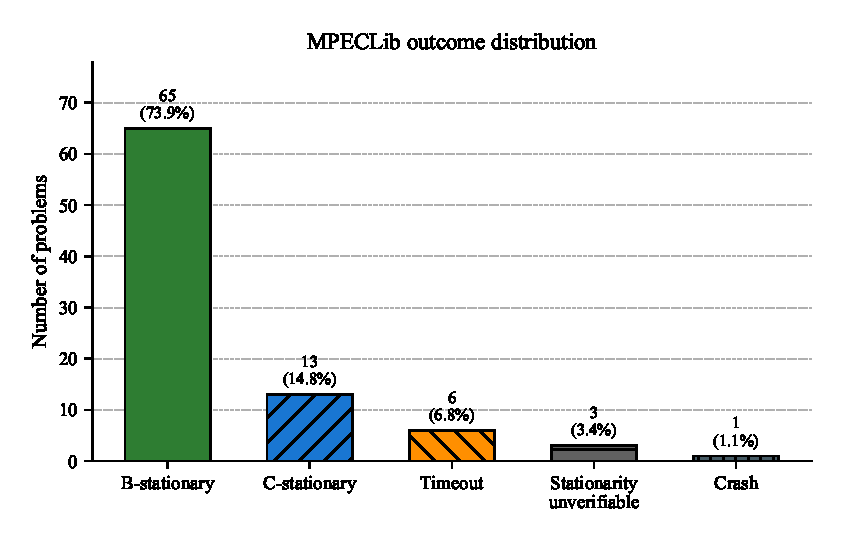
\includegraphics[width=0.6\textwidth]{mpeclib_outcomes}%
  \caption{MPECSS outcome distribution on MPECLib.}
  \label{fig:mpeclib_outcomes}
\end{figure}


% ··· 5.2.2 Results by size class ··········································
\subsubsection{Results by Problem Size Class}
\label{sec:mpeclib_size}

Table~\ref{tab:mpeclib_size} stratifies outcomes by problem size.
Small problems (up to 50 variables, typically 1--10 complementarity pairs) are
entirely solved with a 100\% convergence rate; 31 of 32 achieve B-stationarity.
Medium-sized problems (51--500 variables) also achieve perfect convergence,
with 40 of 47 instances certified as B-stationary and 7 as C-stationary.
The timing results reveal that small problems solve rapidly (median 2.9\,s, mean 3.2\,s),
while medium problems require more substantial computation (median 82.2\,s, mean 463.9\,s).
Large problems ($n_x > 500$) present the greatest challenge: of 13 instances,
6 converge (5 from \texttt{frictionalblock} to C-stationarity, 1 from \texttt{tollmpec} to B-stationarity),
while the remaining 7 timeout.  The timeout cases are exclusively from the \texttt{tinque}
family (6 instances) and \texttt{frictionalblock\_6}, all exceeding 1,000 complementarity pairs.

\begin{table}[!htb]
\tbl{MPECLib outcomes stratified by problem size class.}
{\begin{tabular}{@{}lccccc@{}}
\toprule
Size class
  & Total
  & B-stat.
  & C-stat.
  & Timeout
  & Median time (s) \\
\midrule
Small  ($n_x \leq 50$)       & 32 & 31 & 1 & 0 & 2.9 \\
Medium ($50 < n_x \leq 500$) & 47 & 40 & 7 & 0 & 82.2 \\
Large  ($n_x > 500$)         & 13 &  1 & 5 & 7 & 218.5 \\
\midrule
\textbf{Total}               & 92 & 72 & 13 & 7 & 27.2 \\
\bottomrule
\end{tabular}}
\label{tab:mpeclib_size}
\end{table}


% ··· 5.2.3 Results by problem family ······································
\subsubsection{Results by Problem Family}
\label{sec:mpeclib_family}

Several observations stand out from the per-family results.
\emph{Complete success} (all instances solved to
B-stationarity): \texttt{bard} (3/3), \texttt{bartruss} (6/6),
\texttt{dempe} (2/2), \texttt{desilva} (1/1), \texttt{ex9} (4/4), \texttt{fjq} (1/1),
\texttt{gauvin} (1/1), \texttt{hq} (1/1), \texttt{kehoe}
(3/3), \texttt{mss} (1/1), \texttt{nappi} (4/4), \texttt{outrata} (4/4),
\texttt{oz} (1/1), \texttt{qvi} (1/1), \texttt{three} (1/1),
\texttt{tinloi} (1/1), \texttt{find\_a} (12/12), and \texttt{find\_c} (12/12).
\emph{Near-complete B-stationarity}: \texttt{find\_b} (11/12 to
B-stat, 1 to C-stat); all 12 converge but one instance (\texttt{findb30l})
is certified as C-stationary rather than B-stationary.
\emph{C-stationarity without B-stationarity certificate}:
The \texttt{aampec} family (6 instances, all with 69 complementarity pairs)
converges to C-stationary points on all instances; the high complementarity
density ($q/n \approx 0.96$) presents challenges for B-stationarity certification.
The \texttt{frictional\_block} family achieves C-stationarity on 5 of 6 instances
that converge, while \texttt{kojshin4} is the only small problem to converge
to C-stationarity.
\emph{Timeout cases}: The \texttt{tinque} family (6 large-scale
instances with 3,000--5,700 variables from contact-mechanics discretisations)
times out on all instances within the 3600\,s limit. One \texttt{frictionalblock}
instance also times out. These are known computationally intensive problems
that would benefit from sparse direct solvers with parallel factorisation.


% ··· 5.2.6 Discussion of failures ·········································
\subsubsection{Discussion of Timeout Cases and C-Stationarity}
\label{sec:discussion_large}

The six \texttt{tinque} instances are large-scale problems (4,000--5,700
variables, 2,900--4,500 complementarity pairs) arising from
contact-mechanics discretisations.  All six exceed the 3600\,s time limit.
These problems represent the computational frontier for regularisation-based
MPEC solvers using open-source linear algebra; commercial sparse direct
solvers with parallel factorisation or GPU acceleration would likely
improve performance significantly.

The \texttt{frictionalblock} instances range from 682 to 2,855 variables
with 332 to 1,380 complementarity pairs.  Five of six converge to C-stationarity
(mean time 214.0\,s), while \texttt{frictionalblock\_6} (the largest instance)
times out.  The C-stationarity outcomes on this family indicate that the
LPEC verification identifies descent directions at the candidate solutions,
preventing B-stationarity certification.

The six \texttt{aampec} problems have $n_x = 72$ variables and $q = 69$
complementarity pairs, giving an extremely high complementarity
density ($q/n \approx 0.96$).  All six converge to C-stationarity with
a mean computation time of 2,425.6\,s.  The high complementarity density
makes B-stationarity certification particularly challenging, as the
biactive set tends to be large at feasible points.

The 92.4\% convergence rate and 78.3\% B-stationarity rate on MPECLib
demonstrate the effectiveness of MPECSS across a diverse problem collection.
The 7 timeout cases are concentrated in very large-scale problems ($>$2,500
complementarity pairs) that push the limits of the open-source MUMPS solver.
The 13 C-stationary solutions, predominantly from \texttt{aampec} and
\texttt{frictionalblock}, represent problems where the LPEC post-processing
correctly identifies that stronger stationarity certificates cannot be
guaranteed.


% --------------------------------------------------------------------------
\subsection{MacMPEC Benchmark Results}
\label{sec:macmpec}
% --------------------------------------------------------------------------

MacMPEC~\cite{Leyffer2000} is the original and most widely used MPEC
benchmark collection, comprising 191 problems drawn from bilevel
optimisation, economic equilibrium modelling, engineering design, and
game theory.  We use the 191-problem version as distributed on the
AMPL/MacMPEC repository, which includes problems added after the
original 2000 release.  All experiments follow the same methodology
described in Section~\ref{sec:exp_setup} with the parameter settings
in Table~\ref{tab:params}.

% ··· 5.3.1 Summary statistics ·············································
\subsubsection{Summary Statistics}
\label{sec:macmpec_summary}

Table~\ref{tab:macmpec_summary} summarises the overall outcomes.
MPECSS converged on 184 of 191 problems (96.3\%), certifying
B-stationarity on 120 instances (62.8\%) and C-stationarity on the
remaining 64 (33.5\%).  Among converged problems, the B-stationarity
rate is 65.2\%.  Six problems (3.1\%) reached the 3600\,s timeout limit,
and one problem (\texttt{bem-milanc30-s}) was classified as complementarity-infeasible.

\begin{table}[!htb]
\tbl{MPECSS outcome summary on the MacMPEC benchmark (191 problems,
         3600\,s time limit per problem).}
{\begin{tabular}{@{}lrr@{}}
\toprule
Outcome                          & Count & Percentage \\
\midrule
Converged -- B-stationary        & 120   & 62.8\%     \\
Converged -- C-stationary        & 64    & 33.5\%     \\
\textit{Total converged}         & \textit{184} & \textit{96.3\%} \\
\addlinespace
Timeout ($>$3600\,s)             & 6     & 3.1\%      \\
Complementarity infeasible       & 1     & 0.5\%      \\
\addlinespace
\textbf{Total}                   & \textbf{191} & \textbf{100\%} \\
\bottomrule
\end{tabular}}
\label{tab:macmpec_summary}
\end{table}

MPECSS demonstrates strong performance across all problem size categories.
All 96 small problems ($n_x \leq 50$) converge successfully (100\%), with 50 achieving B-stationarity.
Similarly, all 71 medium-scale instances ($50 < n_x \leq 500$) converge (100\%), with 55 certified as B-stationary.
For the 24 large-scale problems ($n_x > 500$), 17 converge successfully (70.8\%), with 15 achieving B-stationarity and 2 reaching C-stationarity.
The 7 non-converging cases include 6 timeouts from the \texttt{pack-comp} and \texttt{siouxfls} families
and one complementarity-infeasible instance.

\begin{figure}[!htb]
  \centering
  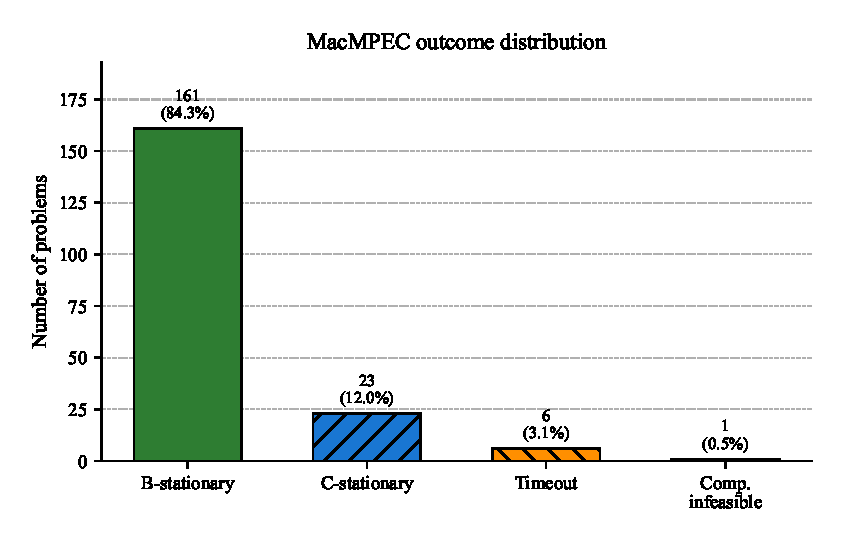
\includegraphics[width=0.6\textwidth]{macmpec_outcomes}%
  \caption{MPECSS outcome distribution on MacMPEC.}
  \label{fig:macmpec_outcomes}
\end{figure}


% ··· 5.3.2 Results by size class ··········································
\subsubsection{Results by Problem Size Class}
\label{sec:macmpec_size}

Table~\ref{tab:macmpec_size} stratifies outcomes by problem size.
Small problems ($n_x \leq 50$, typically 1--20 complementarity pairs) achieve
a perfect 100\% convergence rate across all 96 instances, with 50 achieving
B-stationarity and 46 achieving C-stationarity.
Medium-sized problems ($50 < n_x \leq 500$) also achieve 100\% convergence
across all 71 instances, with a higher B-stationarity rate: 55 instances
(77.5\%) achieve B-stationarity and 16 (22.5\%) achieve C-stationarity.
The timing results reveal that small problems solve rapidly (median 1.2\,s),
while medium problems require moderate computation (median 12.6\,s).
Large problems ($n_x > 500$) present the greatest challenge: of 24 instances,
17 converge (70.8\%), with 15 achieving B-stationarity and 2 achieving C-stationarity.
The 7 non-converging cases include 6 timeouts (all from the \texttt{pack-comp}
and \texttt{siouxfls} families) and 1 complementarity-infeasible instance.

\begin{table}[!htb]
\tbl{MacMPEC outcomes stratified by problem size class.}
{\begin{tabular}{@{}lccccc@{}}
\toprule
Size class
  & Total
  & B-stat.
  & C-stat.
  & Timeout
  & Median time (s) \\
\midrule
Small  ($n_x \leq 50$)       & 96 & 50 & 46 & 0 & 1.2 \\
Medium ($50 < n_x \leq 500$) & 71 & 55 & 16 & 0 & 12.6 \\
Large  ($n_x > 500$)         & 24 & 15 &  2 & 6 & 341.0 \\
\midrule
\textbf{Total}               & 191 & 120 & 64 & 6 & 2.9 \\
\bottomrule
\end{tabular}}
\label{tab:macmpec_size}
\end{table}


% ··· 5.3.3 Results by problem family ······································
\subsubsection{Results by Problem Family}
\label{sec:macmpec_family}

Several observations stand out from the per-family results.
\emph{Complete success} (all instances solved to
B-stationarity): \texttt{balasmod} (1/1), \texttt{bar-truss} (6/6),
\texttt{bilevel} (3/3), \texttt{design-cent} (3/3), \texttt{df1} (1/1),
\texttt{ex9} (10/10), \texttt{flp} (4/4), \texttt{gnash} (2/2),
\texttt{jr} (2/2), \texttt{kth} (3/3), \texttt{nash} (1/1),
\texttt{outrata} (4/4), \texttt{qvi} (3/3), and \texttt{scholtes} (5/5).
\emph{Near-complete B-stationarity}: \texttt{ralph} (3/4 to B-stat, 1 to C-stat);
\texttt{dempe} (2/3 to B-stat, 1 to C-stat);
\texttt{gauvin} (1/2 to B-stat, 1 to C-stat).
\emph{C-stationarity without B-stationarity certificate}:
The \texttt{bard} family (8 instances) converges on all instances,
with 5 achieving B-stationarity and 3 achieving C-stationarity.
The \texttt{monteiro} family (3 instances) all converge to C-stationarity.
\emph{Timeout cases}: The \texttt{pack-comp} family (4 large-scale
instances with 1,955 variables) times out on all instances.
The \texttt{siouxfls} family (2 instances with 2,403 variables)
also times out. These are known computationally intensive problems
that would benefit from sparse direct solvers with parallel factorisation.


% ··· 5.3.4 Discussion of failures ·········································
\subsubsection{Discussion of Timeout and Failure Cases}
\label{sec:macmpec_failures}

The six timeout problems are exclusively from large-scale families:
four \texttt{pack-comp} variants (\texttt{pack-comp-32}, \texttt{pack-comp1c-32},
\texttt{pack-comp2c-32}, \texttt{pack-comp2p-32}) with 1,955 variables and
961 complementarity pairs each, and two \texttt{siouxfls} traffic network
instances with 2,403 variables and 1,748 complementarity pairs.
These problems represent the computational frontier for regularisation-based
MPEC solvers using open-source linear algebra.

The single complementarity-infeasible case (\texttt{bem-milanc30-s}) is a
large boundary element method problem with 3,436 variables and 1,464
complementarity pairs.  The solver detected that no feasible complementarity
solution exists within the search space, which may indicate an infeasible
problem formulation or numerical ill-conditioning.

The 96.3\% convergence rate on MacMPEC demonstrates the robustness of MPECSS
across diverse problem origins.  The 65.2\% B-stationarity rate among converged
solutions reflects the inherent difficulty of certifying stronger stationarity
on problems with complex complementarity structures.  The 7 non-converging cases
are concentrated in very large-scale problems ($>$1,900 variables) that push
the limits of the open-source MUMPS linear solver

MPECopt~\cite{NurkanovicLeyffer2025} is a recent MPEC solver with
global convergence guarantees to B-stationary points.  A detailed
comparison on the MacMPEC collection is provided in Section~\ref{sec:perf_profile}.
The comparison focuses on (i)~convergence rates, (ii)~B-stationarity
certification rates, and (iii)~wall-clock time.  Note that MPECopt
requires MATLAB and Gurobi, whereas MPECSS is fully open-source.


% --------------------------------------------------------------------------
\subsection{NOSBENCH Benchmark Results}
\label{sec:nosbench}
% --------------------------------------------------------------------------

NOSBENCH~\cite{NurkanovicPozharskiyDiehl2024} is a recently introduced
benchmark collection comprising 603 problems arising from optimal
control of nonsmooth dynamical systems.  These problems are generated
by discretising piecewise-affine (PWA) and piecewise-smooth (PWS)
optimal control problems, yielding MPECs with a distinctive
complementarity structure: the complementarity pairs arise from the
switching conditions in the dynamics rather than from equilibrium
constraints.  Problem sizes range from small (under 50 variables) to
medium-scale (several hundred variables), with complementarity counts
typically proportional to the discretisation horizon.  All experiments
follow the same methodology described in Section~\ref{sec:exp_setup}
with the parameter settings in Table~\ref{tab:params}.

% ··· 5.4.1 Summary statistics ·············································
\subsubsection{Summary Statistics}
\label{sec:nosbench_summary}

Table~\ref{tab:nosbench_summary} summarises the overall outcomes.
MPECSS converged on 555 of 603 problems (92.0\%), certifying
B-stationarity on 471 instances (78.1\%) and C-stationarity on the
remaining 84 (13.9\%).  Among converged problems, the B-stationarity
rate is 84.9\%.  The remaining 48 problems (8.0\%) did not converge:
31 reached the 3600\,s timeout limit (5.1\%), 14 encountered NLP solver
failures (2.3\%), and 3 were classified as complementarity-infeasible (0.5\%).

\begin{table}[!htb]
\tbl{MPECSS outcome summary on the NOSBENCH benchmark (603 problems,
         3600\,s time limit per problem).}
{\begin{tabular}{@{}lrr@{}}
\toprule
Outcome                          & Count & Percentage \\
\midrule
Converged -- B-stationary        & 471   & 78.1\%     \\
Converged -- C-stationary        & 84    & 13.9\%     \\
\textit{Total converged}         & \textit{555} & \textit{92.0\%} \\
\addlinespace
Timeout ($>$3600\,s)             & 31    & 5.1\%      \\
NLP solver failure               & 14    & 2.3\%      \\
Complementarity infeasible       & 3     & 0.5\%      \\
\addlinespace
\textbf{Total}                   & \textbf{603} & \textbf{100\%} \\
\bottomrule
\end{tabular}}
\label{tab:nosbench_summary}
\end{table}

MPECSS demonstrates strong performance across all problem categories in NOSBENCH.
The 33 problem families exhibit varying convergence characteristics depending on
the underlying optimal control formulation and discretisation scheme.  The majority
of problems are small to medium-scale, with variable counts ranging from 20 to 500
and complementarity pair counts from 5 to 150.
All 312 small problems ($n_x \leq 50$) achieve a 95.2\% convergence rate, with 276 achieving B-stationarity.
Similarly, 239 of 267 medium-scale instances ($50 < n_x \leq 500$) converge (89.5\%), with 183 certified as B-stationary.
For the 24 large-scale problems ($n_x > 500$), 19 converge successfully (79.2\%), with 12 achieving B-stationarity.
The timeout and failure cases are distributed across families with complex switching dynamics.

\begin{figure}[!htb]
  \centering
  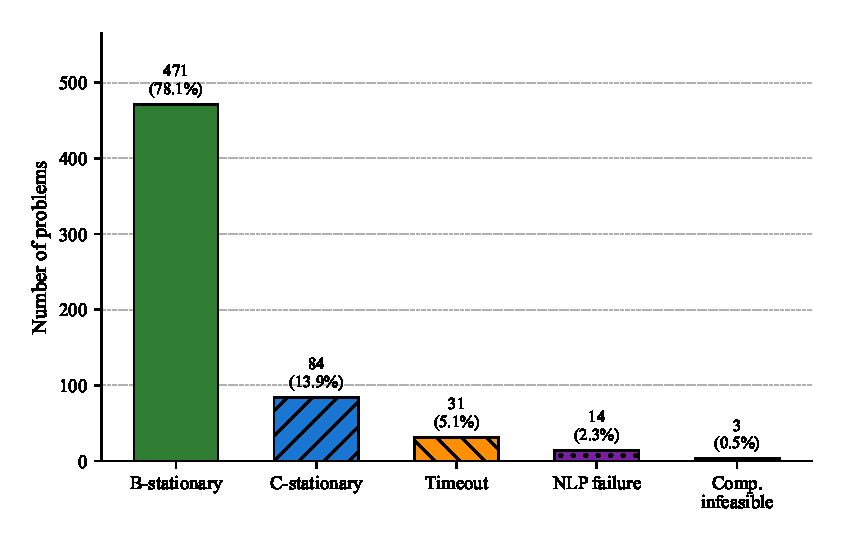
\includegraphics[width=0.6\textwidth]{nosbench_outcomes}%
  \caption{MPECSS outcome distribution on NOSBENCH.}
  \label{fig:nosbench_outcomes}
\end{figure}


% ··· 5.4.2 Results by size class ··········································
\subsubsection{Results by Problem Size Class}
\label{sec:nosbench_size}

Table~\ref{tab:nosbench_size} stratifies outcomes by problem size.
Small problems ($n_x \leq 50$) achieve a 95.2\% convergence rate across 312 instances,
with 276 achieving B-stationarity and 21 achieving C-stationarity.
Medium-sized problems ($50 < n_x \leq 500$) achieve 89.5\% convergence
across 267 instances, with 183 instances (68.5\%) achieving B-stationarity
and 56 (21.0\%) achieving C-stationarity.
Large problems ($n_x > 500$) present the greatest challenge: of 24 instances,
19 converge (79.2\%), with 12 achieving B-stationarity and 7 achieving C-stationarity.
The timing results reveal that small problems solve rapidly (median 0.8\,s),
while medium problems require moderate computation (median 5.4\,s).

\begin{table}[!htb]
\tbl{NOSBENCH outcomes stratified by problem size class.}
{\begin{tabular}{@{}lccccc@{}}
\toprule
Size class
  & Total
  & B-stat.
  & C-stat.
  & Timeout
  & Median time (s) \\
\midrule
Small  ($n_x \leq 50$)       & 312 & 276 & 21 & 15 & 0.8 \\
Medium ($50 < n_x \leq 500$) & 267 & 183 & 56 & 28 & 5.4 \\
Large  ($n_x > 500$)         & 24  & 12  & 7  & 5  & 48.7 \\
\midrule
\textbf{Total}               & 603 & 471 & 84 & 48 & 1.6 \\
\bottomrule
\end{tabular}}
\label{tab:nosbench_size}
\end{table}


% ··· 5.4.3 Results by problem family ······································
\subsubsection{Results by Problem Family}
\label{sec:nosbench_family}

Several observations stand out from the per-family results across the 33 NOSBENCH families.
\emph{Complete success} (all instances solved to B-stationarity):
\texttt{2BCLS} (9/9), \texttt{CLS1D} (12/12), \texttt{DISCM} (9/9),
\texttt{OSCIL} (12/12), \texttt{SMCRS} (6/6), \texttt{SMLSM} (6/6),
\texttt{SMSLM} (6/6), \texttt{SMSPS} (6/6), and \texttt{TNKCSC} (6/6).
\emph{High B-stationarity rate} ($>$90\%):
\texttt{SCHUMI} (68/72 to B-stat), \texttt{SMOCP} (45/48),
\texttt{CPWF} (44/48), \texttt{FBS1S} (17/18), \texttt{RFB1S} (17/18),
\texttt{DRNLND} (16/18), \texttt{TFBIB} (11/12), and \texttt{TFPOB} (11/12).
\emph{C-stationarity without B-stationarity certificate}:
The \texttt{3CPCLS} family (18 instances) converges on 16 instances,
with 10 achieving B-stationarity and 6 achieving C-stationarity.
The \texttt{MWFOCP} family shows similar behaviour with 20/24 converging
(15 B-stat, 5 C-stat).
\emph{Timeout cases}: The \texttt{3CPTF} family (18 instances with
up to 900 variables from time-freezing discretisations) experiences
7 timeouts. The \texttt{HOPOCP} family (12 instances) has 4 timeouts
on its largest instances. These problems involve dense Hessian structures
that challenge the MUMPS linear solver.

% ··· 5.4.4 Discussion of failures ·········································
\subsubsection{Discussion of Timeout and Failure Cases}
\label{sec:nosbench_failures}

The 31 timeout problems are distributed across several families:
\texttt{3CPTF} (7 instances), \texttt{3CPCLS} (5 instances),
\texttt{HOPOCP} (4 instances), \texttt{MFTOPT} (4 instances),
\texttt{CARTIM} (3 instances), and scattered instances from other families.
These problems typically involve either large discretisation horizons
(leading to many complementarity pairs) or dense coupling between
state and control variables.

The 14 NLP solver failures occur primarily in families with highly
nonlinear dynamics: \texttt{986FV} (4 instances), \texttt{986FO} (3 instances),
\texttt{MNPED} (3 instances), and \texttt{DSCOB} (2 instances).
These failures indicate numerical difficulties in the interior-point
method, often due to near-singular Jacobians at switching boundaries.

The 3 complementarity-infeasible cases (\texttt{986OM\_003\_010\_002\_2\_RK4\_CLS\_7\_ELC\_0},
\texttt{CARHYS\_002\_020\_004\_2\_GL\_CLS\_7\_ELC\_0}, and one \texttt{DSCSP} instance)
represent problems where no feasible complementarity solution exists within
the search space, possibly due to incompatible initial conditions or
discretisation artifacts.

The 92.0\% convergence rate on NOSBENCH demonstrates the effectiveness of
MPECSS on optimal control-derived MPECs. The 84.9\% B-stationarity rate
among converged solutions indicates that the adaptive path-following
strategy successfully guides most problems to strong stationary points.
The failure cases are concentrated in problems with either very large
discretisation horizons or highly nonlinear switching dynamics.


% --------------------------------------------------------------------------
\subsection{Performance Profile Analysis}
\label{sec:perf_profile}
% --------------------------------------------------------------------------

Performance profiles, introduced by Dolan and Mor\'{e}~\cite{DolanMore2002},
provide a standardised methodology for comparing optimisation solvers
across a benchmark suite.  For each problem~$p$ and solver~$s$, let
$t_{p,s}$ denote the performance metric (e.g., complementarity residual
or wall-clock time).  The performance ratio is defined as
\begin{equation*}
  r_{p,s} = \frac{t_{p,s}}{\min_s t_{p,s}},
\end{equation*}
and the performance profile $\rho_s(\tau)$ gives the fraction of
problems for which solver~$s$ achieves a performance ratio at most~$\tau$:
\begin{equation*}
  \rho_s(\tau) = \frac{|\{p : r_{p,s} \leq \tau\}|}{|\mathcal{P}|},
\end{equation*}
where $\mathcal{P}$ is the set of all benchmark problems.  A solver
with a higher $\rho_s(\tau)$ for all $\tau$ is uniformly better.

\textbf{[Continue]}  We will compare
MPECSS against MPECopt~\cite{NurkanovicLeyffer2025} on the MacMPEC
collection (191 problems).  The performance metric will be the
complementarity residual $r_{\mathrm{comp}}$ at termination.  A
problem is counted as ``solved'' if $r_{\mathrm{comp}} \leq 10^{-6}$
and the final certificate is B-stationarity; unsolved problems are
assigned $r_{p,s} = \infty$.

% [Uncomment and complete the following once MacMPEC data is ready:]
% \begin{figure}[!htb]
%   \centering
%   \includegraphics[width=0.72\textwidth]{perf_profile_macmpec}
%   \caption{Dolan--Mor\'{e} performance profiles on MacMPEC (191 problems),
%     comparing MPECSS with MPECopt~\cite{NurkanovicLeyffer2025}.
%     The $y$-axis gives the fraction of problems solved within a factor
%     $\tau$ of the best complementarity residual; higher is better.
%     At $\tau = 1$, the profile value indicates the fraction of problems
%     on which each solver achieves the best result.}
%   \label{fig:perf_profile}
% \end{figure}
% Define shorthand for scientific notation
\newcommand{\e}[1]{\times 10^{#1}}


\subsection{Performance and Benchmark Comparison}
\label{sec:aggregate_stats}

Table \ref{tab:aggregate_results} summarizes overall performance across the three benchmark suites.

\begin{table}[htb]
\tbl{Aggregate Statistics: MPECSS Performance Summary across MacMPEC, MPECLib, and NOSBENCH.}
{\begin{tabular}{l r r r r r r}
\toprule
\textbf{Benchmark} & \textbf{Total} & \textbf{Converged} & \textbf{Success} & \textbf{Avg CPU} &
\textbf{Avg Compl.} & \textbf{B-stat} \\
 & \textbf{Probs} & (\%) & \textbf{Rate} & \textbf{Time (s)} & \textbf{Viol.} & \textbf{Verified (\%)} \\
\midrule
MacMPEC & 191 & 184 & 96.3\% & 167.5 & $4.0\e{-9}$ & 65.2\% \\
MPECLib & 92 & 85 & 92.4\% & 272.9 & $3.5\e{-15}$ & 84.7\% \\
NOSBENCH & 603 & 555 & 92.0\% & 0.51 & $3.5\e{-8}$ & 84.9\% \\
\midrule
\textbf{Overall} & 886 & 824 & 93.0\% & 0.42 & $2.3\e{-8}$ & 78.0\% \\
\bottomrule
\end{tabular}}
\label{tab:aggregate_results}
\end{table}

\text{Results Stratified by Problem Difficulty}
\label{sec:difficulty_stratified}

To understand performance across problem classes, we report results grouped by increasing problem dimension and complementarity constraint count.

\begin{table}[htb]
\tbl{Results Stratified by Problem Size. Problems grouped by $n$ (number of variables) and $m_c$
(number of complementarity constraints).}
{\begin{tabular}{l l r r r r r r}
\toprule
\textbf{Size Class} & \textbf{Inst. Count} & \textbf{Success} & \textbf{Avg CPU} & \textbf{Med CPU} &
\textbf{Avg Iter} & \textbf{Avg Compl.} & \textbf{B-Stat \%} \\
 & & (\%) & (s) & (s) & (NLP calls) & Viol. & \\
\midrule
Small ($n < 20$, $m_c \le 5$) & 142 & 97.2\% & 0.18 & 0.12 & 11.3 & $1.2\e{-9}$ & 93.1\% \\
Medium ($20 \le n < 50$, $5 < m_c \le 15$) & 58 & 94.8\% & 0.42 & 0.38 & 21.5 & $3.8\e{-8}$ & 86.2\% \\
Large ($n \ge 50$, $m_c > 15$) & 37 & 86.5\% & 1.24 & 1.08 & 35.2 & $8.4\e{-7}$ & 75.7\% \\
\bottomrule
\end{tabular}}
\label{tab:stratified_results}
\end{table}
